\documentclass{article}
\usepackage[utf8]{inputenc}
\usepackage{xcolor}
\usepackage{mdframed}
\usepackage{graphicx}
\graphicspath{ {./img/} }

\title{OpenVASP: An Open Protocol to Implement FATF's
Travel Rule for Virtual Assets}
\author{David Riegelnig, Bitcoin Suisse}
\date{November 14, 2019}

\usepackage{natbib}
\usepackage{graphicx}

\begin{document}

\maketitle

\section*{Summary}
In June 2019, the Financial Action Task Force (FATF) issued updated guidance on "Virtual Assets and Virtual Asset Service Providers"\footnote{ http://www.fatf-gafi.org/publications/fatfrecommendations/documents/public-statement-virtual-assets.html}, providing additional clarifications on how its recommendations should be understood in the context of virtual asset transactions. Implementation of the newest recommendations is under way in some countries\footnote{E.g. in Switzerland: Anti-Money Laundering Ordinance (AMLO-FINMA), issued by Swiss Financial Market Supervisory Authority (FINMA), in particular Article 10; FINMA Guidance 02/2019 Payments on the blockchain}, yet for most FATF members, awareness of the requirement is still in the very early stages.

The FATF has been monitoring and providing guidance on money laundering and terrorism financing prevention since 2014. In 2018, the international body adopted changes to its recommendations to define "virtual assets" and introduced the term "virtual asset service provider" (VASP). Yet, the implementation of some of the most recent guidance is a challenge for the still nascent crypto-financial industry. Recommendation 16, often referred to as "Travel Rule", presents particular challenges, requiring industry participants to agree on common standards. It requires any VASP to obtain, hold, and transmit originator and beneficiary information when conducting virtual asset transactions with obliged entities as defined by the FATF (other VASPs, banks and financial intermediaries).

This white paper outlines an open protocol among VASPs for the mutual exchange of originator and beneficiary information. It does so in a fully decentralized manner, leveraging cryptographically secure peer-to-peer communication and capabilities of the Ethereum blockchain for authentication. The protocol works with any blockchain or distributed ledger technology (DLT) used for the underlying virtual asset transfer. It puts privacy of transferred data at the center of its design.
The protocol facilitates robust compliance, purely based on a set of principles for VASPs around the world, regardless of jurisdiction or technology used and without membership or registration with a centralized third-party. It is meant as a contribution to the ongoing dialogue of members of the crypto-financial community and regulators around the globe.

\newpage
\tableofcontents
\newpage


\section{Overview}

\subsection*{Design Principles (Chapter 2)}
An outline of the seven design principles guiding the protocol's design.

\subsection*{Messaging Layer (Chapter 3)}
Requirements are defined for the underlying asynchronous communication layer so that the protocol can possibly be implemented on top of different existing messaging systems. The Whisper protocol is introduced as an exemplary peer-to-peer messaging layer.

\subsection*{Addressing (Chapter 4)}
Making sure the protocol works with any blockchain or distributed ledger system used for the underlying virtual asset transfer, including upcoming Layer 2 solutions, a generic addressing and routing system is required. We introduce the Virtual Assets Account Number (VAAN), which borrows elements from proven payment routing systems (such as the IBAN), without compromising on the decentralized approach.

\subsection*{Authentication (Chapter 5)}
Robust end-to-end encryption requires strong mutual authentication between VASPs in the first place. The protocol leverages the Ethereum blockchain as a public key infrastructure, avoiding the known weaknesses of central certificate authorities. Mutual authentication between VASPs is at the center of the protocol's trust model, complemented by attestations from trusted third parties like self-regulatory organizations and trade associations.

\subsection*{Protocol Flow (Chapter 6)}
The protocol defines a simple flow of steps to facilitate a structured communication between two VASPs transferring virtual assets on behalf of their respective customers.

\subsection*{Protocol Messages (Chapter 7)}
A set of structured messages is specified, which borrows proven elements from modern payment standards (i.e. ISO 20022), tailored for the specific needs arising for VASPs.

\newpage

    
\section{Design Principles}
In designing this proposal for an open protocol to facilitate compliance with FATF's travel rule for virtual assets, we were guided by the following seven principles.

% hide subsections from ToC but keep numbering
\addtocontents{toc}{\protect\setcounter{tocdepth}{1}}

\subsection{Travel Rule Compliance}
    \begin{mdframed}[backgroundcolor=gray!20] 
        Establish a shared communication protocol for VASPs to exchange virtual asset transfer information as specified in the FATF requirements.
    \end{mdframed}
This principle includes:
\renewcommand{\theenumi}{\alph{enumi}}
 \begin{enumerate}
   \item a common transfer data standard for required originator and beneficiary information;
   \item a suitable set of rules to facilitate the data exchange between VASPs.
  \end{enumerate}
 
\subsection{Decentralized Approach}
    \begin{mdframed}[backgroundcolor=gray!20] 
    Pursue a decentralized approach that enables any two VASPs to use the protocol without consent or even knowledge of any third party.
    \end{mdframed}
This principle includes that the protocol:
\renewcommand{\theenumi}{\alph{enumi}}
 \begin{enumerate}
   \item does not require a VASP to obtain any form of membership or registration with any third party;
   \item does not require the usage of a central component at any time;
   \item assumes that each VASP has a non-delegable obligation to carefully select other VASPs it wants to work with, following a risk-based approach.
  \end{enumerate}
  
\subsection{Technology Agnostic}
    \begin{mdframed}[backgroundcolor=gray!20] 
    Make sure the protocol works with any blockchain or distributed ledger technology (DLT) used for the underlying virtual asset transfer.
    \end{mdframed}
This principle includes that the protocol:
\renewcommand{\theenumi}{\alph{enumi}}
 \begin{enumerate}
   \item requires no changes to the underlying blockchain / DLT;
   \item does not assume specific characteristics of the underlying blockchain / DLT (e.g. the existence of a unique identifier or comment field in transactions).
  \end{enumerate}
  \newpage
  
\subsection{Privacy by Design}
    \begin{mdframed}[backgroundcolor=gray!20] 
    Make sure the protocol puts privacy of transferred data at the center of its design.
    \end{mdframed}
This principle includes that the protocol:
\renewcommand{\theenumi}{\alph{enumi}}
 \begin{enumerate}
   \item requires robust authentication of the VASPs involved;
   \item requires robust end-to-end encryption between VASPs;
   \item applies perfect forward secrecy (protecting data transferred in the past against future compromises of the private keys);
   \item allows for two VASPs to transfer data without the knowledge of any third party.
  \end{enumerate}
  
\subsection{Broad Applicability}
    \begin{mdframed}[backgroundcolor=gray!20] 
    Ensure that the protocol facilitates all applicable usage scenarios where VASPs need to exchange transfer data.
    \end{mdframed}
This principle includes that the protocol:
\renewcommand{\theenumi}{\alph{enumi}}
 \begin{enumerate}
   \item supports VASPs exchanging data as part of a one-off virtual asset transfer;
   \item supports VASPs exchanging data for a high number of routine transactions;
   \item supports situations where the beneficiary VASP is not known to the sending VASP or where there is uncertainty whether a target address is controlled by a VASP;
   \item supports situations where virtual asset transfers between VASPs are initiated or facilitated by smart contracts.
  \end{enumerate}
  
\subsection{Extensibility}
    \begin{mdframed}[backgroundcolor=gray!20] 
    Ensure that the protocol allows for custom extensions.
    \end{mdframed}
This principle includes that the protocol:
\renewcommand{\theenumi}{\alph{enumi}}
 \begin{enumerate}
   \item allows for VASPs to add custom data;
   \item while doing so, has rules that prevent any weakening of the common core.
  \end{enumerate}
  \newpage
  
\subsection{Efficient to Use}
    \begin{mdframed}[backgroundcolor=gray!20] 
    Ensure minimal cost for VASPs to deploy and maintain the protocol's implementation.
    \end{mdframed}
This principle includes that the protocol:
\renewcommand{\theenumi}{\alph{enumi}}
 \begin{enumerate}
   \item supports straight-through processing capabilities;
   \item supports implementations where a single server instance can process virtual asset transfers in all blockchains / DLTs used by the VASP.
  \end{enumerate}

% close subsection-ToC-hiding
%\addtocontents{toc}{\protect\setcounter{tocdepth}{2}}

\newpage

\section{Messaging Layer}

\subsection{Generic requirements}
On the underlying communication layer, the protocol requires to send and receive asynchronous messages in simple datagram format.
    \begin{mdframed}[backgroundcolor=gray!20]
    \begin{tabular}{ l l }
    \multicolumn{2}{ l }{ \texttt{[Header,Data]} }\\
    \verb+Header+:&Addressing information \& reference for receiver how to \\
    &decrypt the data (4 bytes)  \\  
    \verb+Data+:&Encrypted message content    
    \end{tabular}
    \end{mdframed}
    
The proposed architecture does not assume a secure connection between sender and receiver and is therefore not requiring the messaging layer to handle authentication. Instead, the protocol defines a communication handshake based on structured messages, where the session key used for subsequent encryption is generated.

Addressing is based on the VASP's unique identity (for initial handshake) and the session (for subsequent messages). Again, no specific requirements are imposed on the messaging layer, allowing for different approaches how routing is implemented.

Details on addressing, session handling and message structure are described in further chapters.

\subsection{Range of possible underlying messaging protocols}

Given these minimal requirements, a wide range of underlying messaging protocols could be used, which is helpful in supporting a wide range of usage scenarios.

To illustrate this, one could utilize standard unencrypted email to exchange protocol messages, simply using the subject field for header information and the email body for data. Doing so is not very efficient and would be vulnerable to traffic analysis, albeit only regarding the identity of the sender and the receiver, but it would still work. Naturally, any other direct connection between sender and receiver being able to exchange messages specified above can be used.

However, in line with its decentralized approach, the protocol is designed to work with a peer-to-peer communication layer as well. In such a system, each node passes on every message it receives to some (gossiping) or all (flooding) of its neighbors. Routing works because the receiving node can decide based on the message header, whether he is the addressee and then try to decrypt the message data with his private key or a previously agreed shared key.

Ideally, a set of initially supported messaging layers will be part of the final protocol specification, following broader discussion with industry participants. For this paper, Whisper is taken as an exemplary peer-to-peer protocol.

\subsection{Ethereum Whisper as an example}

The Whisper messaging system has been developed as part of the Ethereum technology stack but can be used separately from the blockchain. It was designed to provide resilience and strong privacy in a peer-to-peer environment and targets message delivery below five seconds on a global scale.

Given the design goals for the OpenVASP protocol, Whisper seems a good fit with its focus on secure, untraceable communication between peers. It benefits from using Ethereum’s proven network layer and is available for all to use. Adoption will be facilitated for VASPs already running Ethereum nodes.

The reader is recommended to consult the online documentation about the Whisper protocol\footnote{https://geth.ethereum.org/docs/whisper/whisper-overview}. Hence, the following sections provide just a brief overview about Whisper and its key functionality, partially citing from the mentioned source.

\subsubsection{Functionality}
\noindent\normalsize\textbf{3.3.1.1 Resilience and Privacy}

Whisper has been designed as a peer-to-peer messaging system with focus on resilience and privacy. As a matter of principle, a Whisper message is sent to every Whisper node and every message is encrypted by default. The one who can decrypt the message, is the intended recipient. That way, Whisper can ideally provide absolute anonymity for the recipient. However, nodes can choose their level of anonymity by leaking limited information for better performance if so desired.

As each node passes on all incoming messages, neighboring nodes learn nothing about the origin of a message. In addition, a node can send random messages to maintain a constant level of “noise”. Therefore, Whisper protects the sender as well, even in case of a powerful adversary attempting to do targeted traffic analysis.

\vspace{1em}
\noindent\normalsize\textbf{3.3.1.2	Dark Routing}

Decrypting every incoming message would put a too heavy strain on computational resources. For this reason, Whisper messages include a 4-byte “topic”, which is a probabilistic hint for the recipient to watch out for and to try to decrypt. The receiver can subscribe to several topics along with the respective symmetric and asymmetric key.

The occurrence of collisions, meaning that a receiver attempts to decrypt a message with a matching topic to find out it cannot be decrypted as it was for another receiver, are deliberate to ensure plausible deniability.


\vspace{1em}
\noindent\normalsize\textbf{3.3.1.3	Latency}

It has been designed for message delivery below five seconds.
\newpage

\vspace{1em}
\noindent\normalsize\textbf{3.3.1.4	Time-to-live (TTL)}

When sending a Whisper message, the sender decides on a time-to-live (specified in seconds) with a maximum time span of two days. Messages are kept in every Whisper node until their TTL expires. When a new node connects, it will receive all messages whose TTL has not yet expired. The Whisper network is therefore storing a message for a specific time, which is useful in situations when a node has a short downtime.

\vspace{1em}
\noindent\normalsize\textbf{3.3.1.5	Protection from denial-of-service attacks}

To protect the Whisper network from denial-of-service attacks, sending a message requires a proof-of-work to be accepted by any forwarding node. The required proof-of-work is proportional to both message size and TTL.

\vspace{1em}
\noindent\normalsize\textbf{3.3.1.6	Encryption}

Every Whisper message is encrypted either symmetrically or asymmetrically. Messages can be decrypted by anyone who possesses the corresponding key.

Asymmetric encryption uses the standard Elliptic Curve Integrated Encryption Scheme with SECP-256k1 public key. Symmetric encryption uses AES GCM algorithm with random 96-bit nonce.

\vspace{1em}
\noindent\normalsize\textbf{3.3.1.7	Underlying transport layer}

Whisper is implemented on top of the RLPx, a TCP-based transport protocol also used for communication among Ethereum nodes.

\subsubsection{Whisper envelopes and messages}
Envelopes are the packets sent and received by Whisper nodes. They contain the encrypted message and metadata for decryption. Once decoded, they have the following format:
    \begin{mdframed}[backgroundcolor=gray!20] 
    \begin{tabular}{ l l }
        \multicolumn{2}{ l }{ \texttt{[Version, Expiry, TTL, Topic, AESNonce, Data, EnvNonce]} }\\
        \verb+Expiry time+:& 4 bytes (UNIX time in seconds)\\
        \verb+TTL+:&4 bytes (time-to-live in seconds)\\
        \verb+Topic+:&4 bytes of arbitrary data\\
        \verb+AESNonce+:&12 bytes of random data(in case of symmetric encryption)\\
        \verb+Data+:&byte array of arbitrary size(contains encrypted message)\\
        \verb+EnvNonce+:&8 bytes of arbitrary data(used for PoW calculation)
    \end{tabular}
    \end{mdframed}
    
Upon receipt of a message, if the node detects a known topic, it tries to decrypt the message with the corresponding symmetric and asymmetric key. In case of failure, the node assumes that topic collision occurs, e.g. the message was encrypted with another key. If decryption is successful, the message is revealed with the following structure:

    \begin{mdframed}[backgroundcolor=gray!20] 
     \begin{tabular}{ l l }
    \verb+Flags+:&	1 byte\\
    \verb+Padding+:& byte array of arbitrary size, optional\\
    \verb+Message+:& byte array of arbitrary size (actual message content)\\
    \verb+Signature+:& 65 bytes, optional, Ethereum ECDSA signature\\
    &(Keccak-256 hash of unencrypted data)\\
    \end{tabular}
    \end{mdframed}
    
Those unable to decrypt the message data are also unable to access the signature.
\newpage

\section{Addressing}
\subsection{VASP identity \& VASP code}
The protocol uses the Ethereum blockchain as a decentralized public-key infrastructure (see next chapter). Each participating VASP must deploy a standardized smart contract, which represents its identity on the blockchain, similar to how a traditional public key certificate would function.

The Ethereum address of the standardized smart contract deployed by a VASP is defined to be the VASP identity and the last 32 bits are called VASP code. Both values are numbers encoded as hexadecimals, which are easy to process and human-readable. However, the “0x” radix, typically used to indicate the hexadecimal format, is omitted for the VASP code.

\begin{figure}[h]
    \centering
    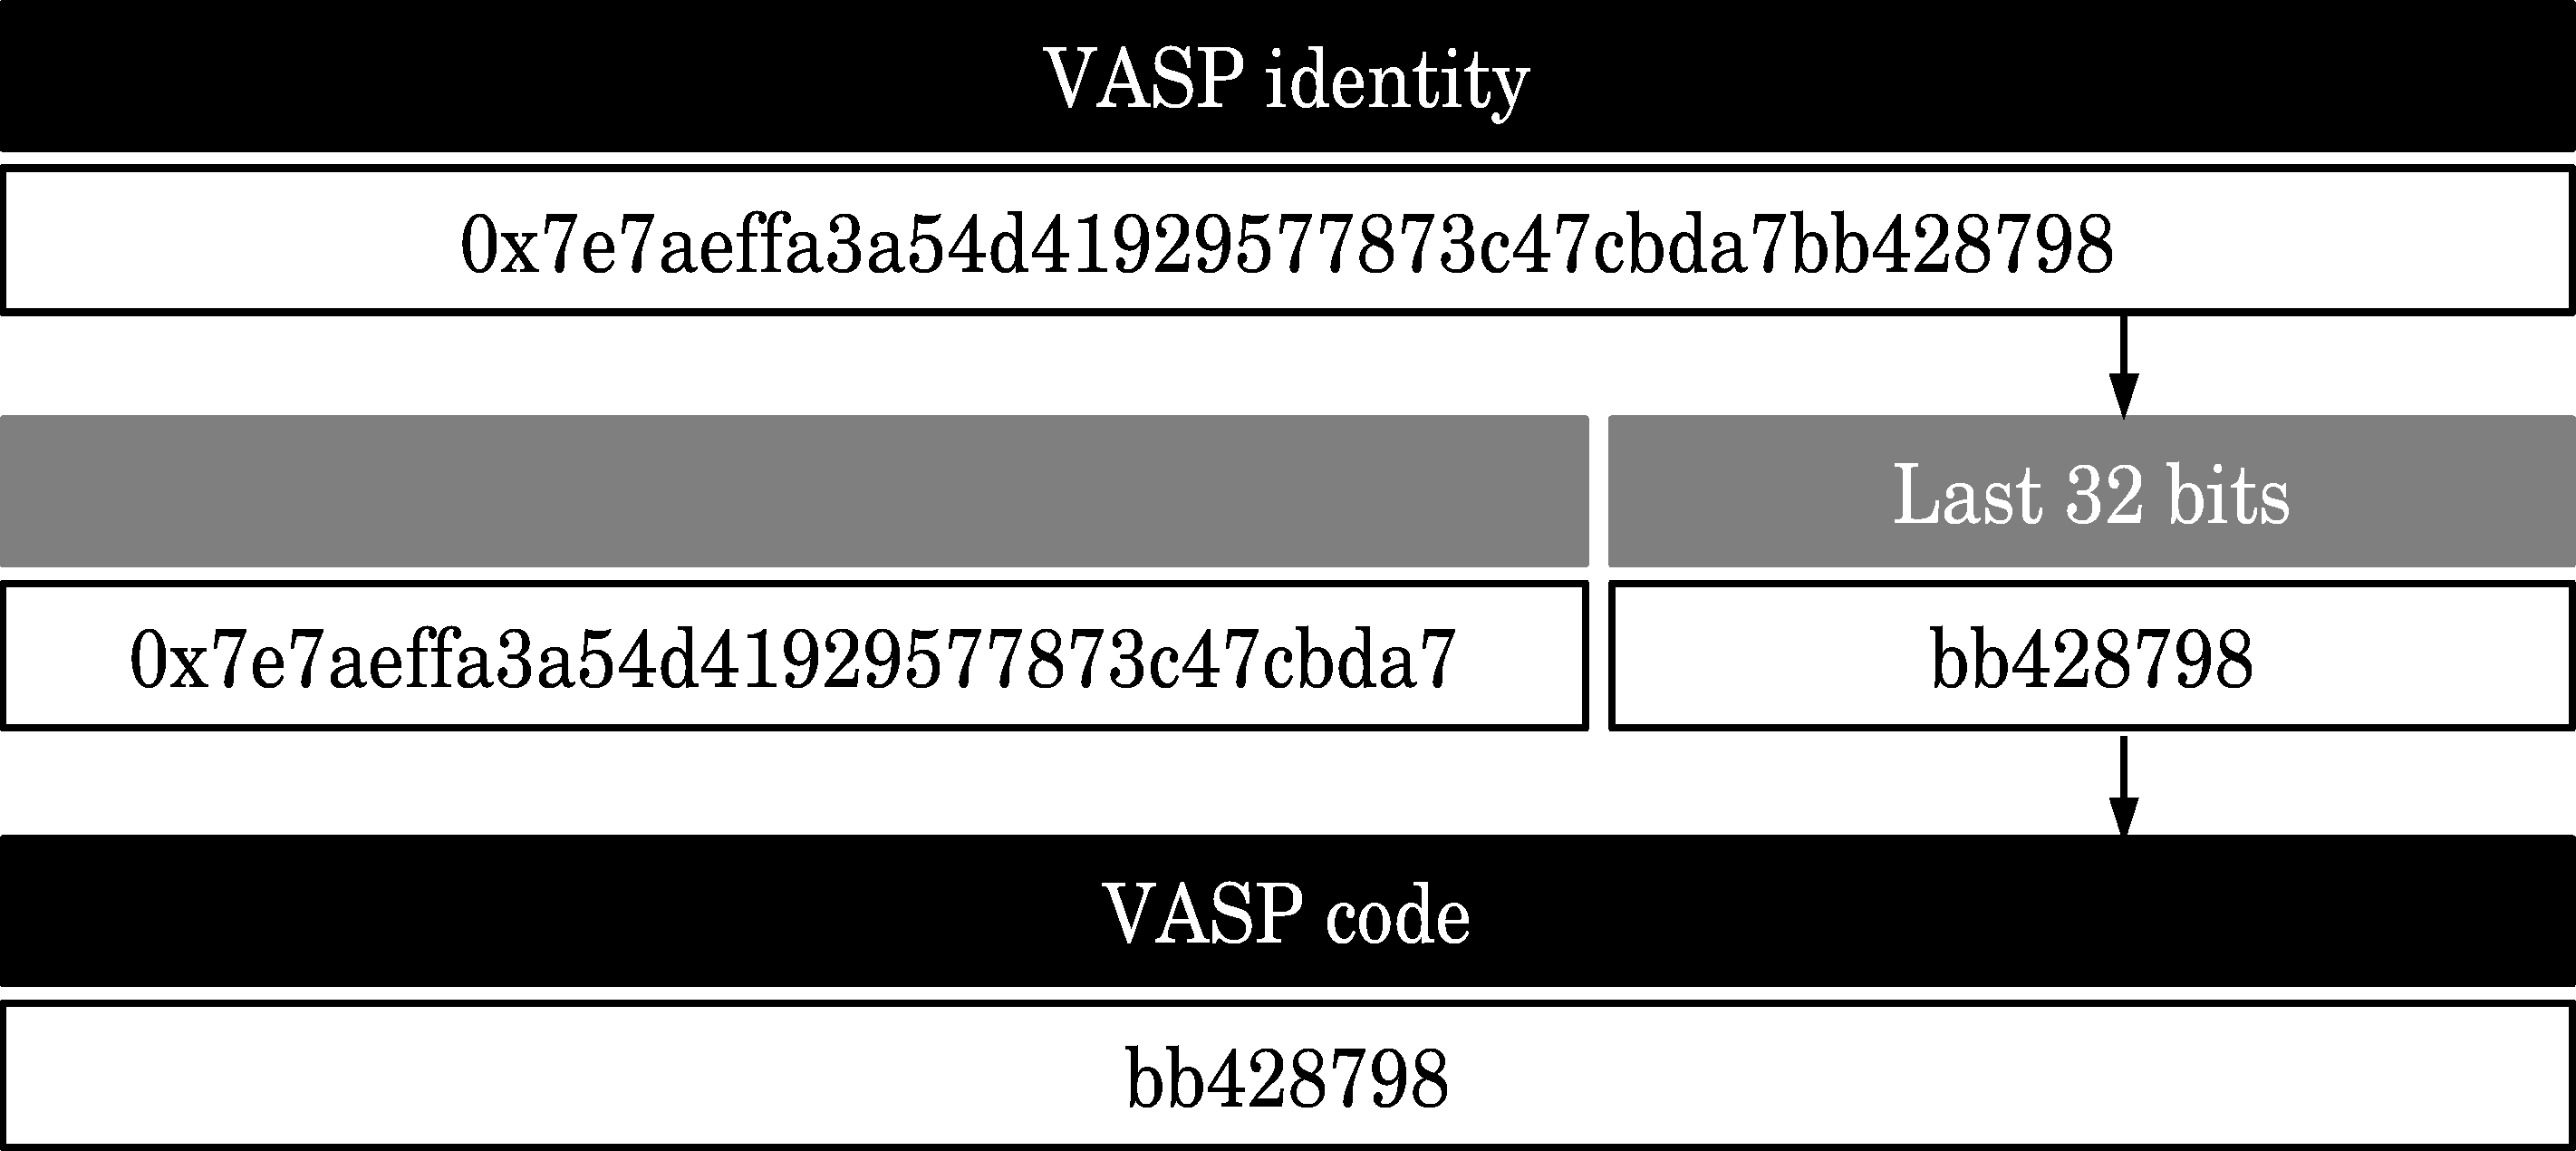
\includegraphics[width=0.75\textwidth]{g1.pdf}
\end{figure}


\subsection{Virtual Assets Account Number (VAAN)}
At the outset, the beneficiary wants to receive virtual assets on a wallet hosted by a VASP and therefore provides the originator with routing information on where to send them. The originator then instructs his VASP to transfer the virtual assets based on the routing information.

In traditional payment systems, bank account numbers in combination with bank identifiers (e.g. BIC/SWIFT, IBAN) are used as routing information.

We suggest a similar, but decentralized approach in form of the Virtual Assets Account Number (VAAN), which is a 24-character hex code including a 2-character checksum. The leading eight characters correspond to the VASP code, while the remaining characters are customer specific.

The VAAN should not contain spaces when transmitted electronically. When printed, it can be expressed in groups of four characters separated by a single space for readability.

\begin{figure}[h]
    \centering
    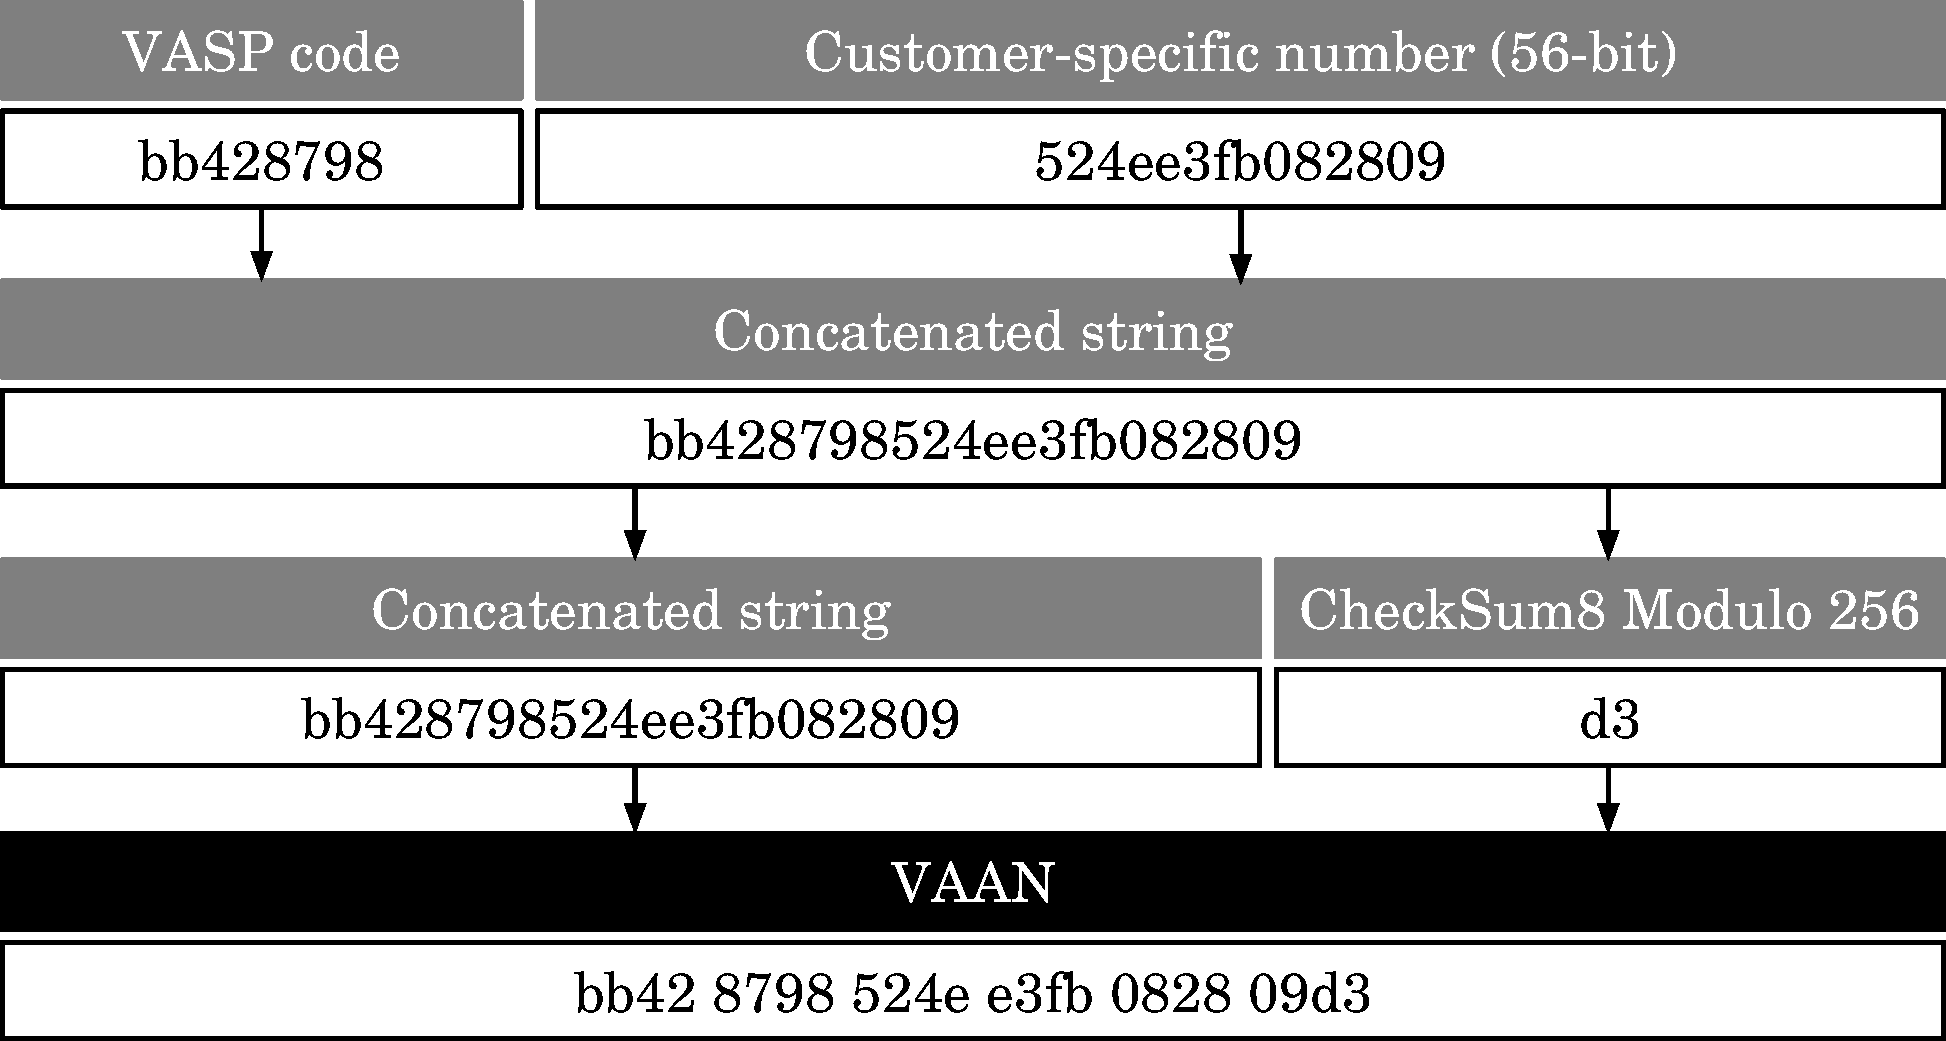
\includegraphics[width=0.75\textwidth]{g2.pdf}
\end{figure}

It is at the discretion of each VASP to define the details of how VAANs are assigned and used by their customers. The proposed length of 14 hex characters (56 bits) for the client-specific number of the VAAN gives each VASP a sufficiently large address space of $7.2\times1016$ identifiers, allowing plenty of room including vanity numbers.

A VASP could assign a single, fixed VAAN to each customer by default, similar to how a traditional bank account number is used. Another VASP might provide multiple VAANs on request or limit their period of validity. Privacy-minded customers might even prefer to use a VAAN only once.

While VASPs are completely free in assigning VAANs to their customers within the boundaries of the format, they must ensure that each VAAN is uniquely assigned to exactly one of their customers. By doing so, the regulatory requirement for unique identification is ensured.

The proposed format allows the VAAN to be exchanged easily (e.g. via email) between beneficiary and originator and facilitates VASP-to-VASP transfers of virtual assets beyond the purpose of FATF compliance.

\subsection{VAAN-based message routing}
The VASP code, being the first 8 characters of the VAAN, is used as the header to send messages to the respective VASP.

In case of Whisper, the header (VASP code) can directly be used as topic to route message envelopes to the receiver (see previous chapter).

\vspace{1em}
\begin{figure}[h]
    \centering
    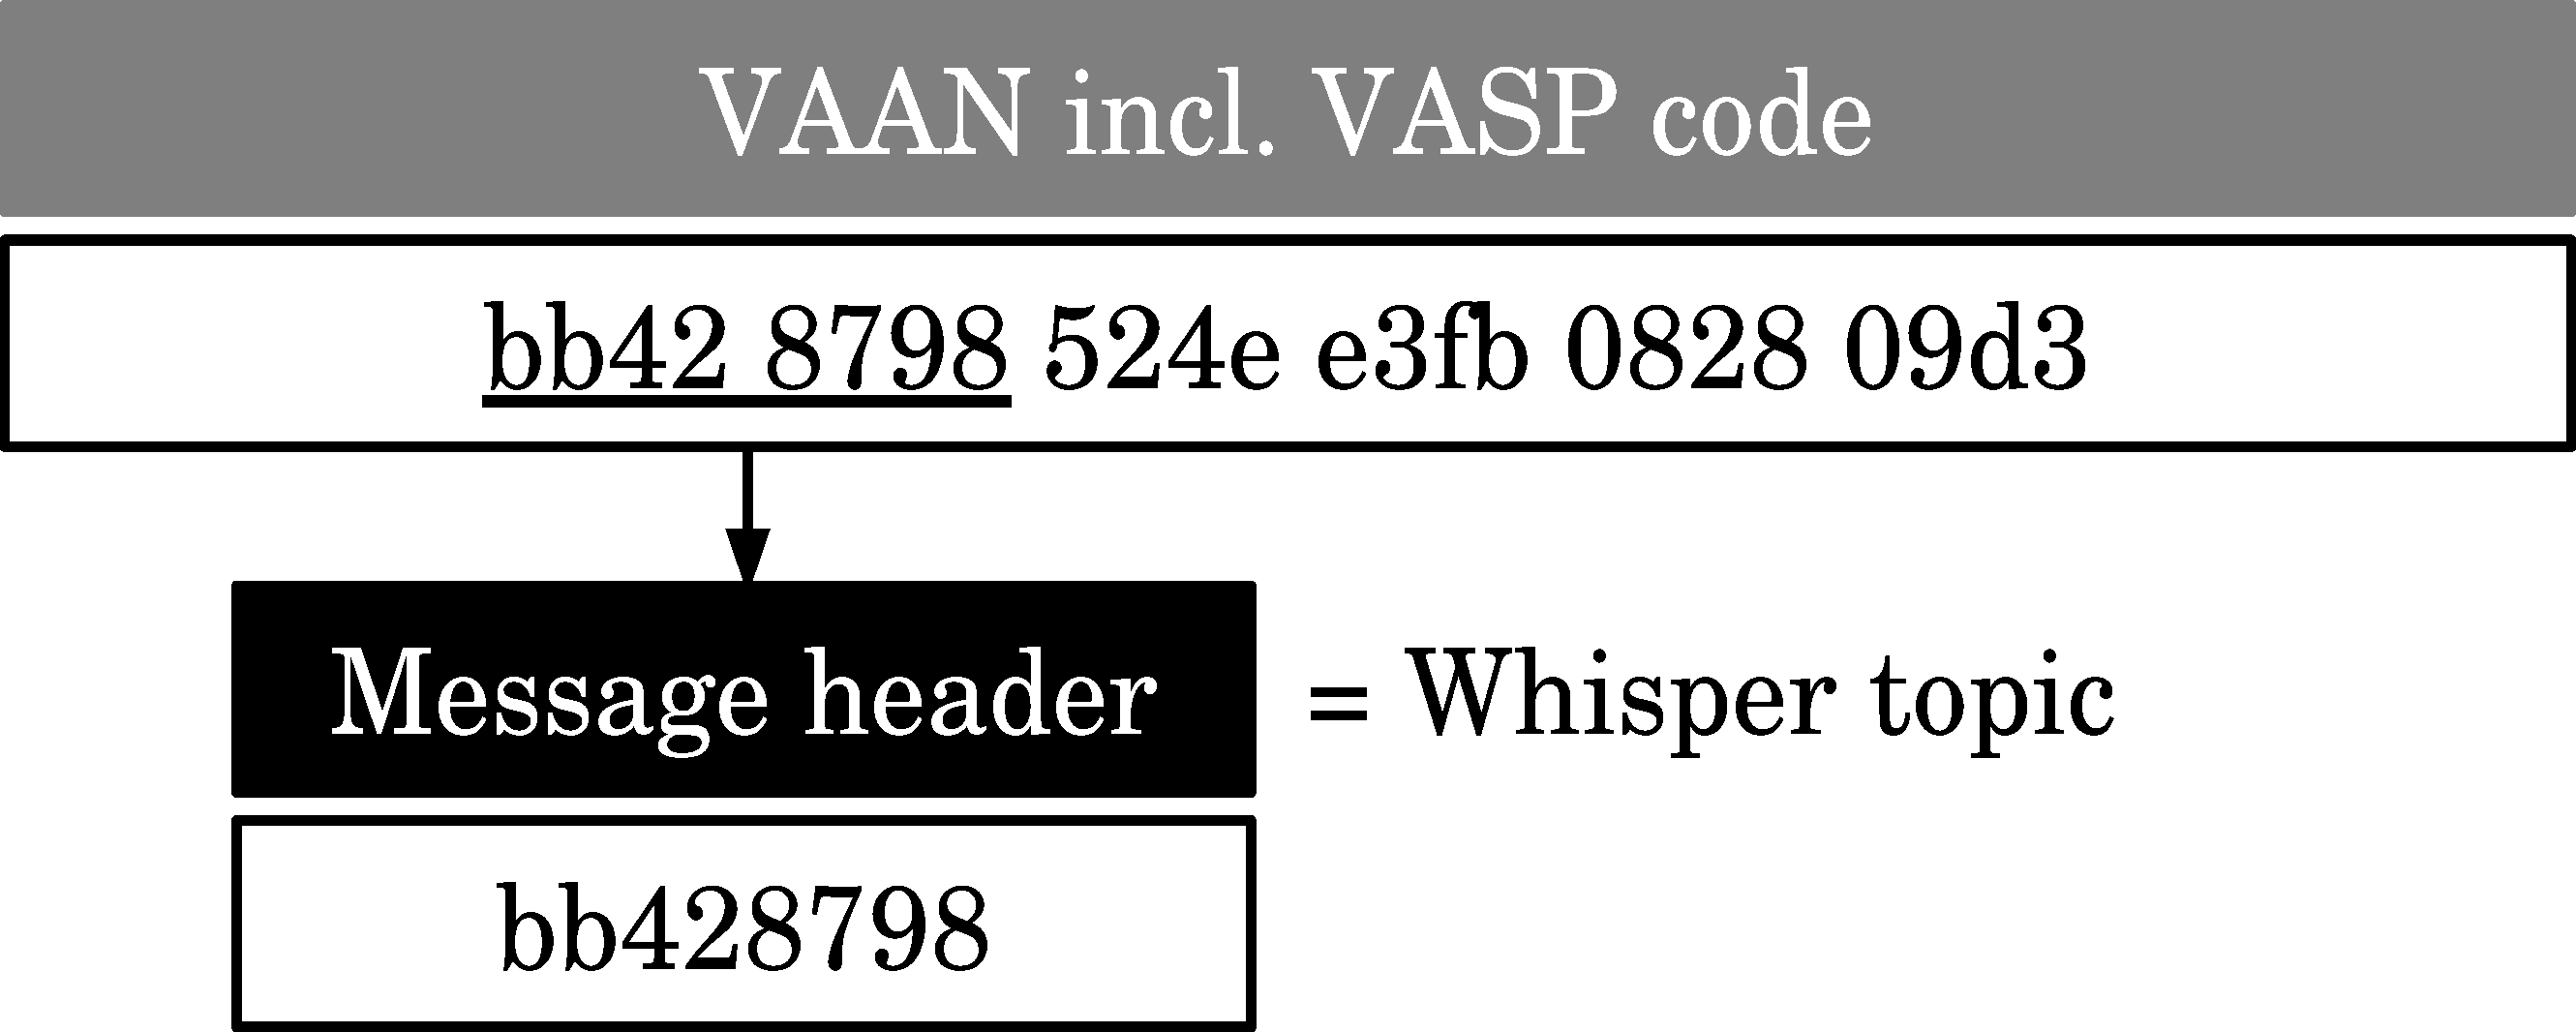
\includegraphics[width=0.5\textwidth]{g3.pdf}
\end{figure}
\newpage

\subsection{Transfer instructions to be given by a customer}
From a customers’ perspective, only the name and the VAAN have to be provided to receive virtual assets to his/her wallet hosted by a VASP.

\begin{figure}[h]
    \centering
    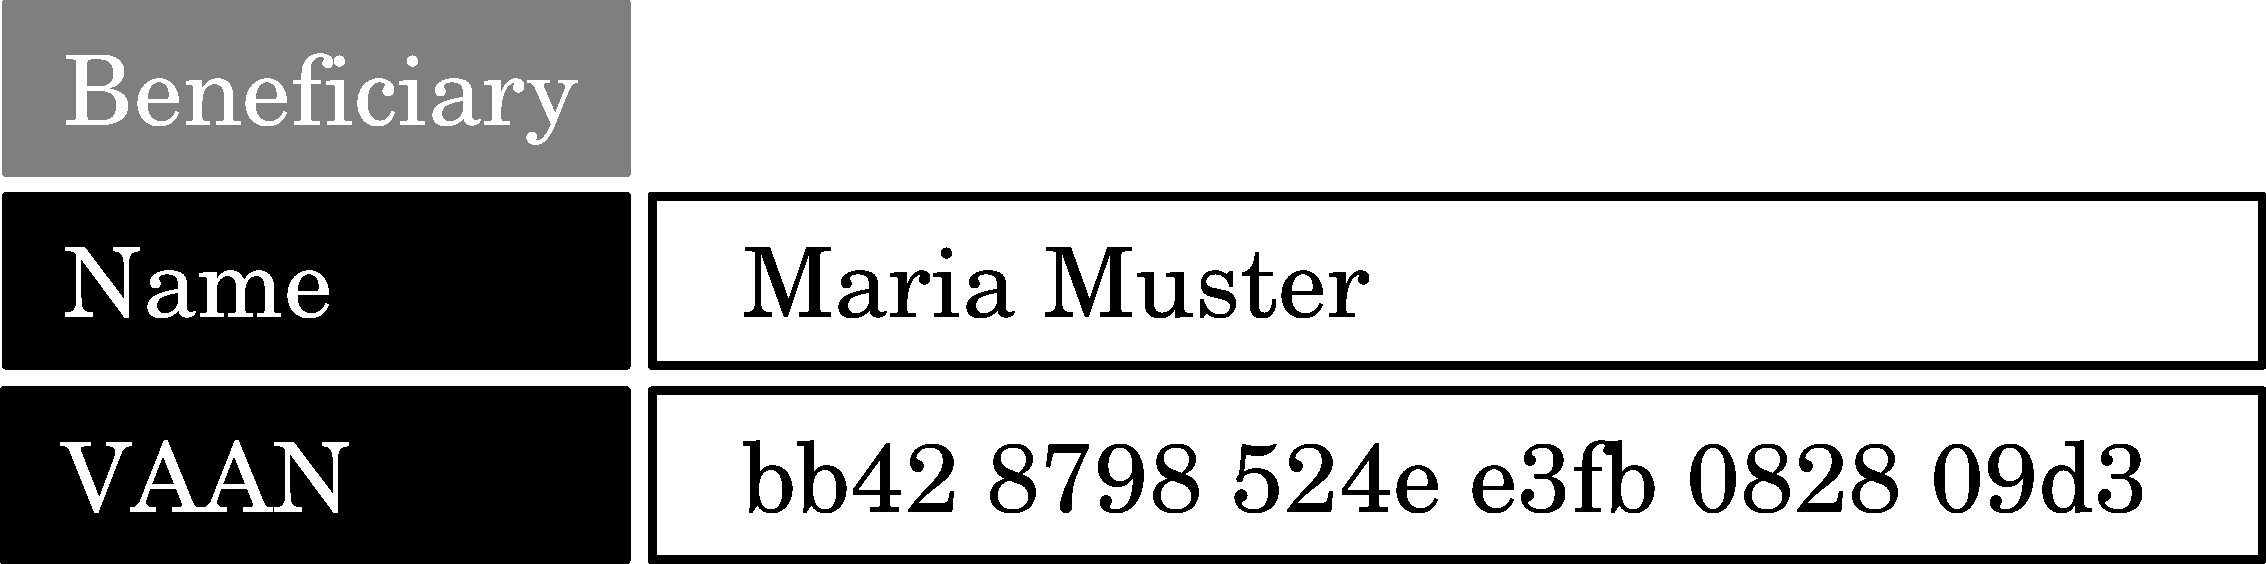
\includegraphics[width=0.5\textwidth]{g4.pdf}
\end{figure}
\newpage

\section{Authentication}
A standardized Ethereum smart contract (called VASP contract) is used to represent the identity of a VASP. Each VASP deploys its own contract and can also withdraw it at any time. As described in the previous chapter (section 4.1), the Ethereum address of the contract is defined to be the VASP identity.

\subsection{Direct and indirect authentication among VASPs}

Direct mutual authentication between counterparty VASPs forms the basis of the protocol’s trust model. Whenever two VASPs establish their business relationship, their respective identities can be directly authenticated, meaning first-hand evidence is available that the other VASP’s identity is genuine. For significant VASP-to-VASP relationships with virtual asset transfers occurring regularly (e.g. broker/exchange, bank/custodian) authenticating each other’s identity will happen as part of the usual onboarding process between financial intermediaries. While there is no requirement to make this step public, most VASPs will find visible recognition from reputable counterparties to be a sign of good standing.

Certified authentication by trusted third parties is the protocol’s second approach to ensure robust authentication. Recognized self-regulatory organizations and trade associations are particularly suitable to issue identity claims for their respective members. Claims by such issuers can directly include an attestation about the VASP’s license or registration status obtained from competent authorities.

Identity claims made by either peer VASPs or trusted issuers are signed and recorded in the VASP contract for everyone’s reference. Claims can also be revoked by the issuing party at any time.

\begin{figure}[h]
    \centering
    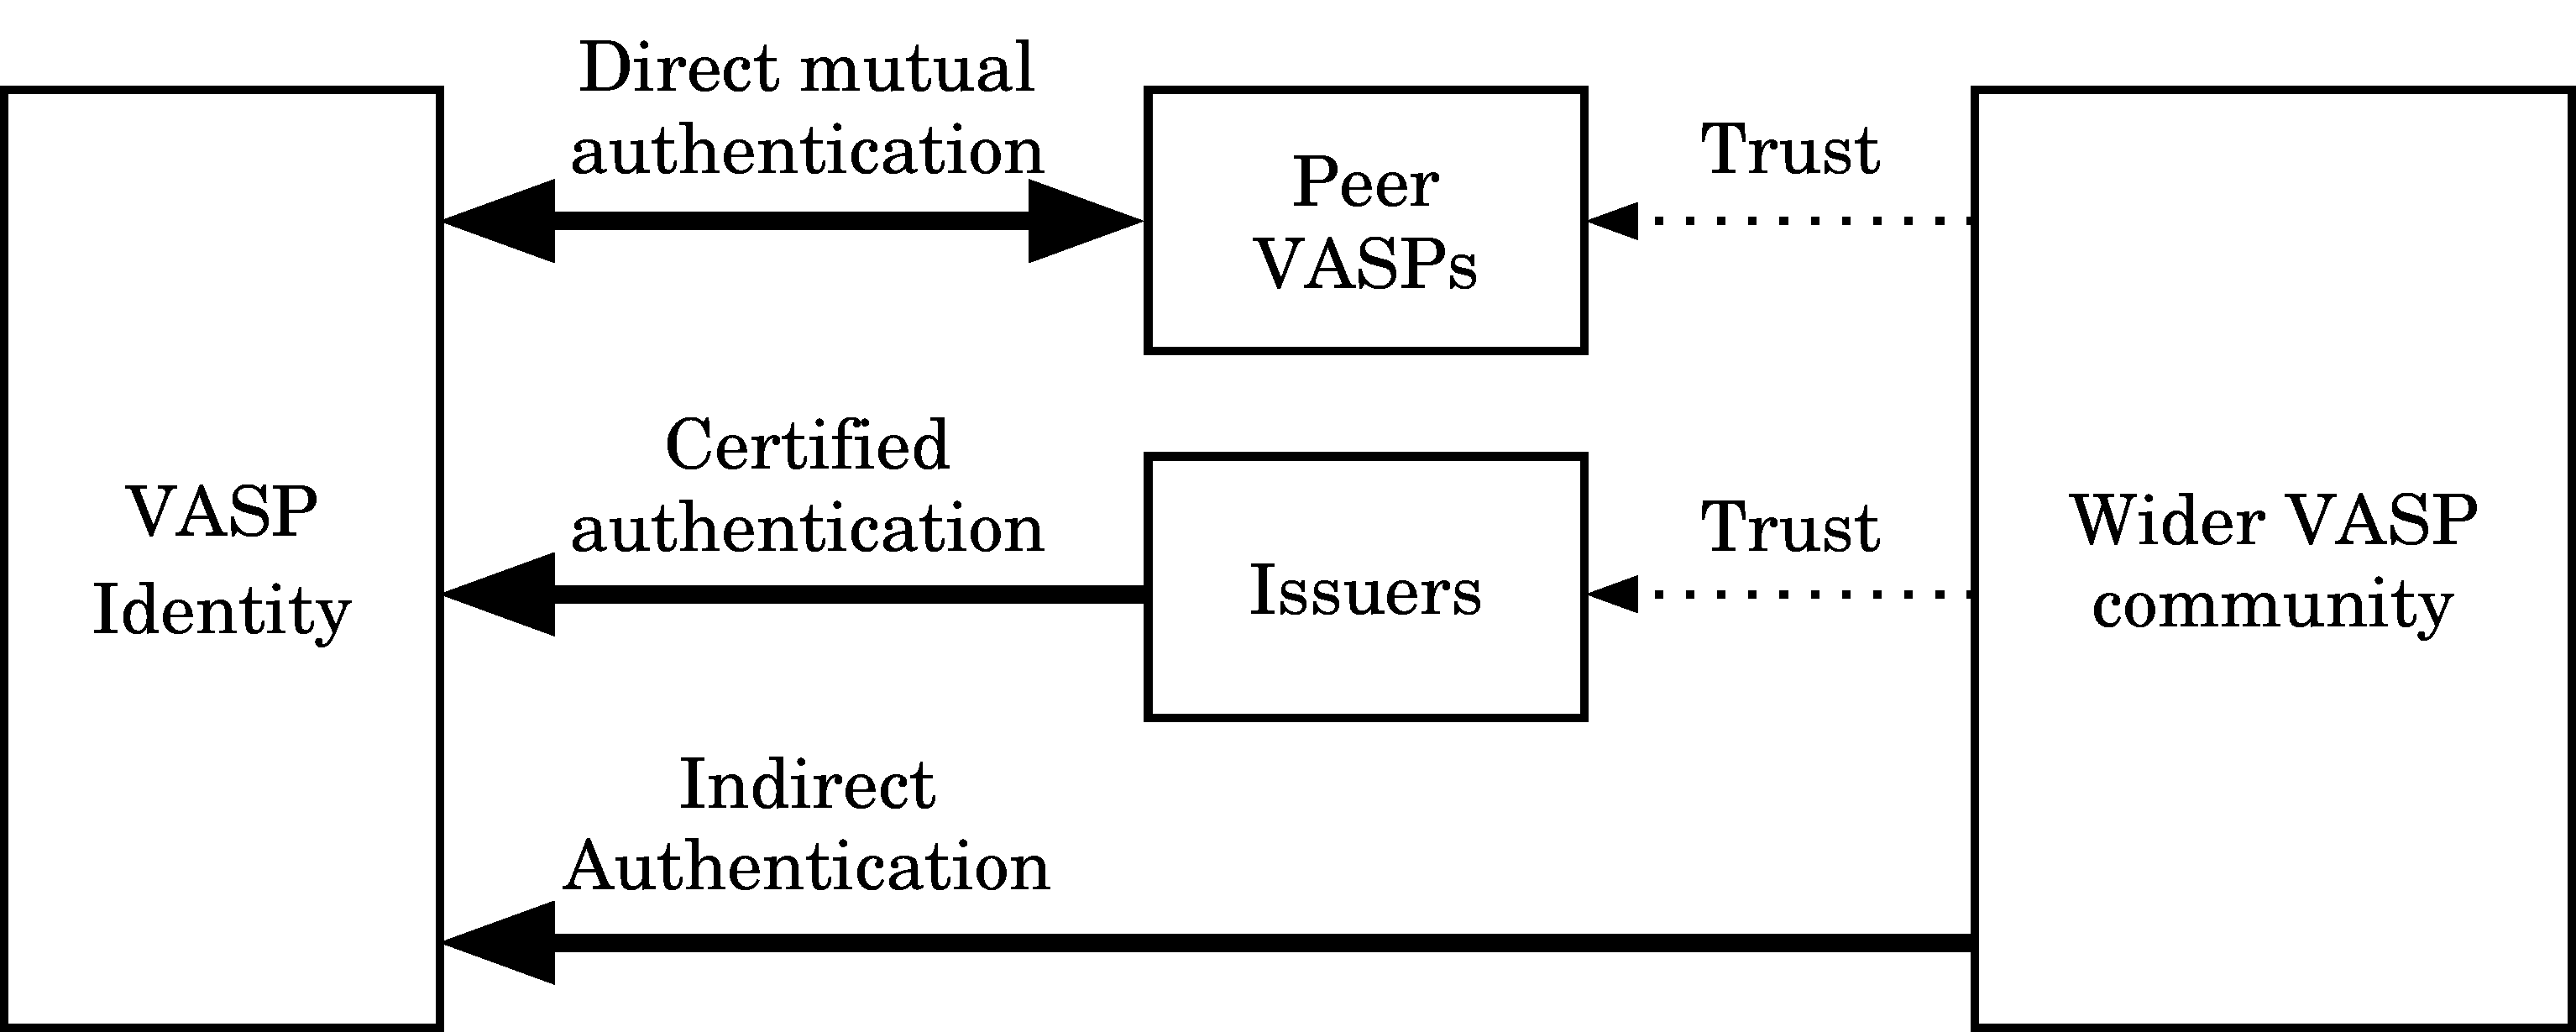
\includegraphics[width=0.75\textwidth]{g5.pdf}
\end{figure}

The ability to retrieve proven identity claims about a VASP on the blockchain at any time, enables the wider community of VASPs to partially rely on indirect trust relationships. While risk-based decision making is required, indirect authentication will be often feasible for one-time transfers of moderate value.


\subsection{VASP contract}

A high-level specification of the VASP contract is outlined in this section, focusing on the most important aspects required for the functioning of the protocol.
As mentioned earlier, each VASP deploys its own contract instance and takes the contracts’ deployment address as identity identifier and the last 32 bits as the VASP code. The contract includes relevant information about the VASP.

For better security and to facilitate separation of duties, different roles should be implemented (e.g. owner, administrator). Addresses assigned to these roles can again point to multi-sig smart contracts for better security. However, the VASP contract itself should be as simple as possible and delegate access control and governance to calling contracts and systems.
\vspace{2em}
\begin{figure}[h]
    \centering
    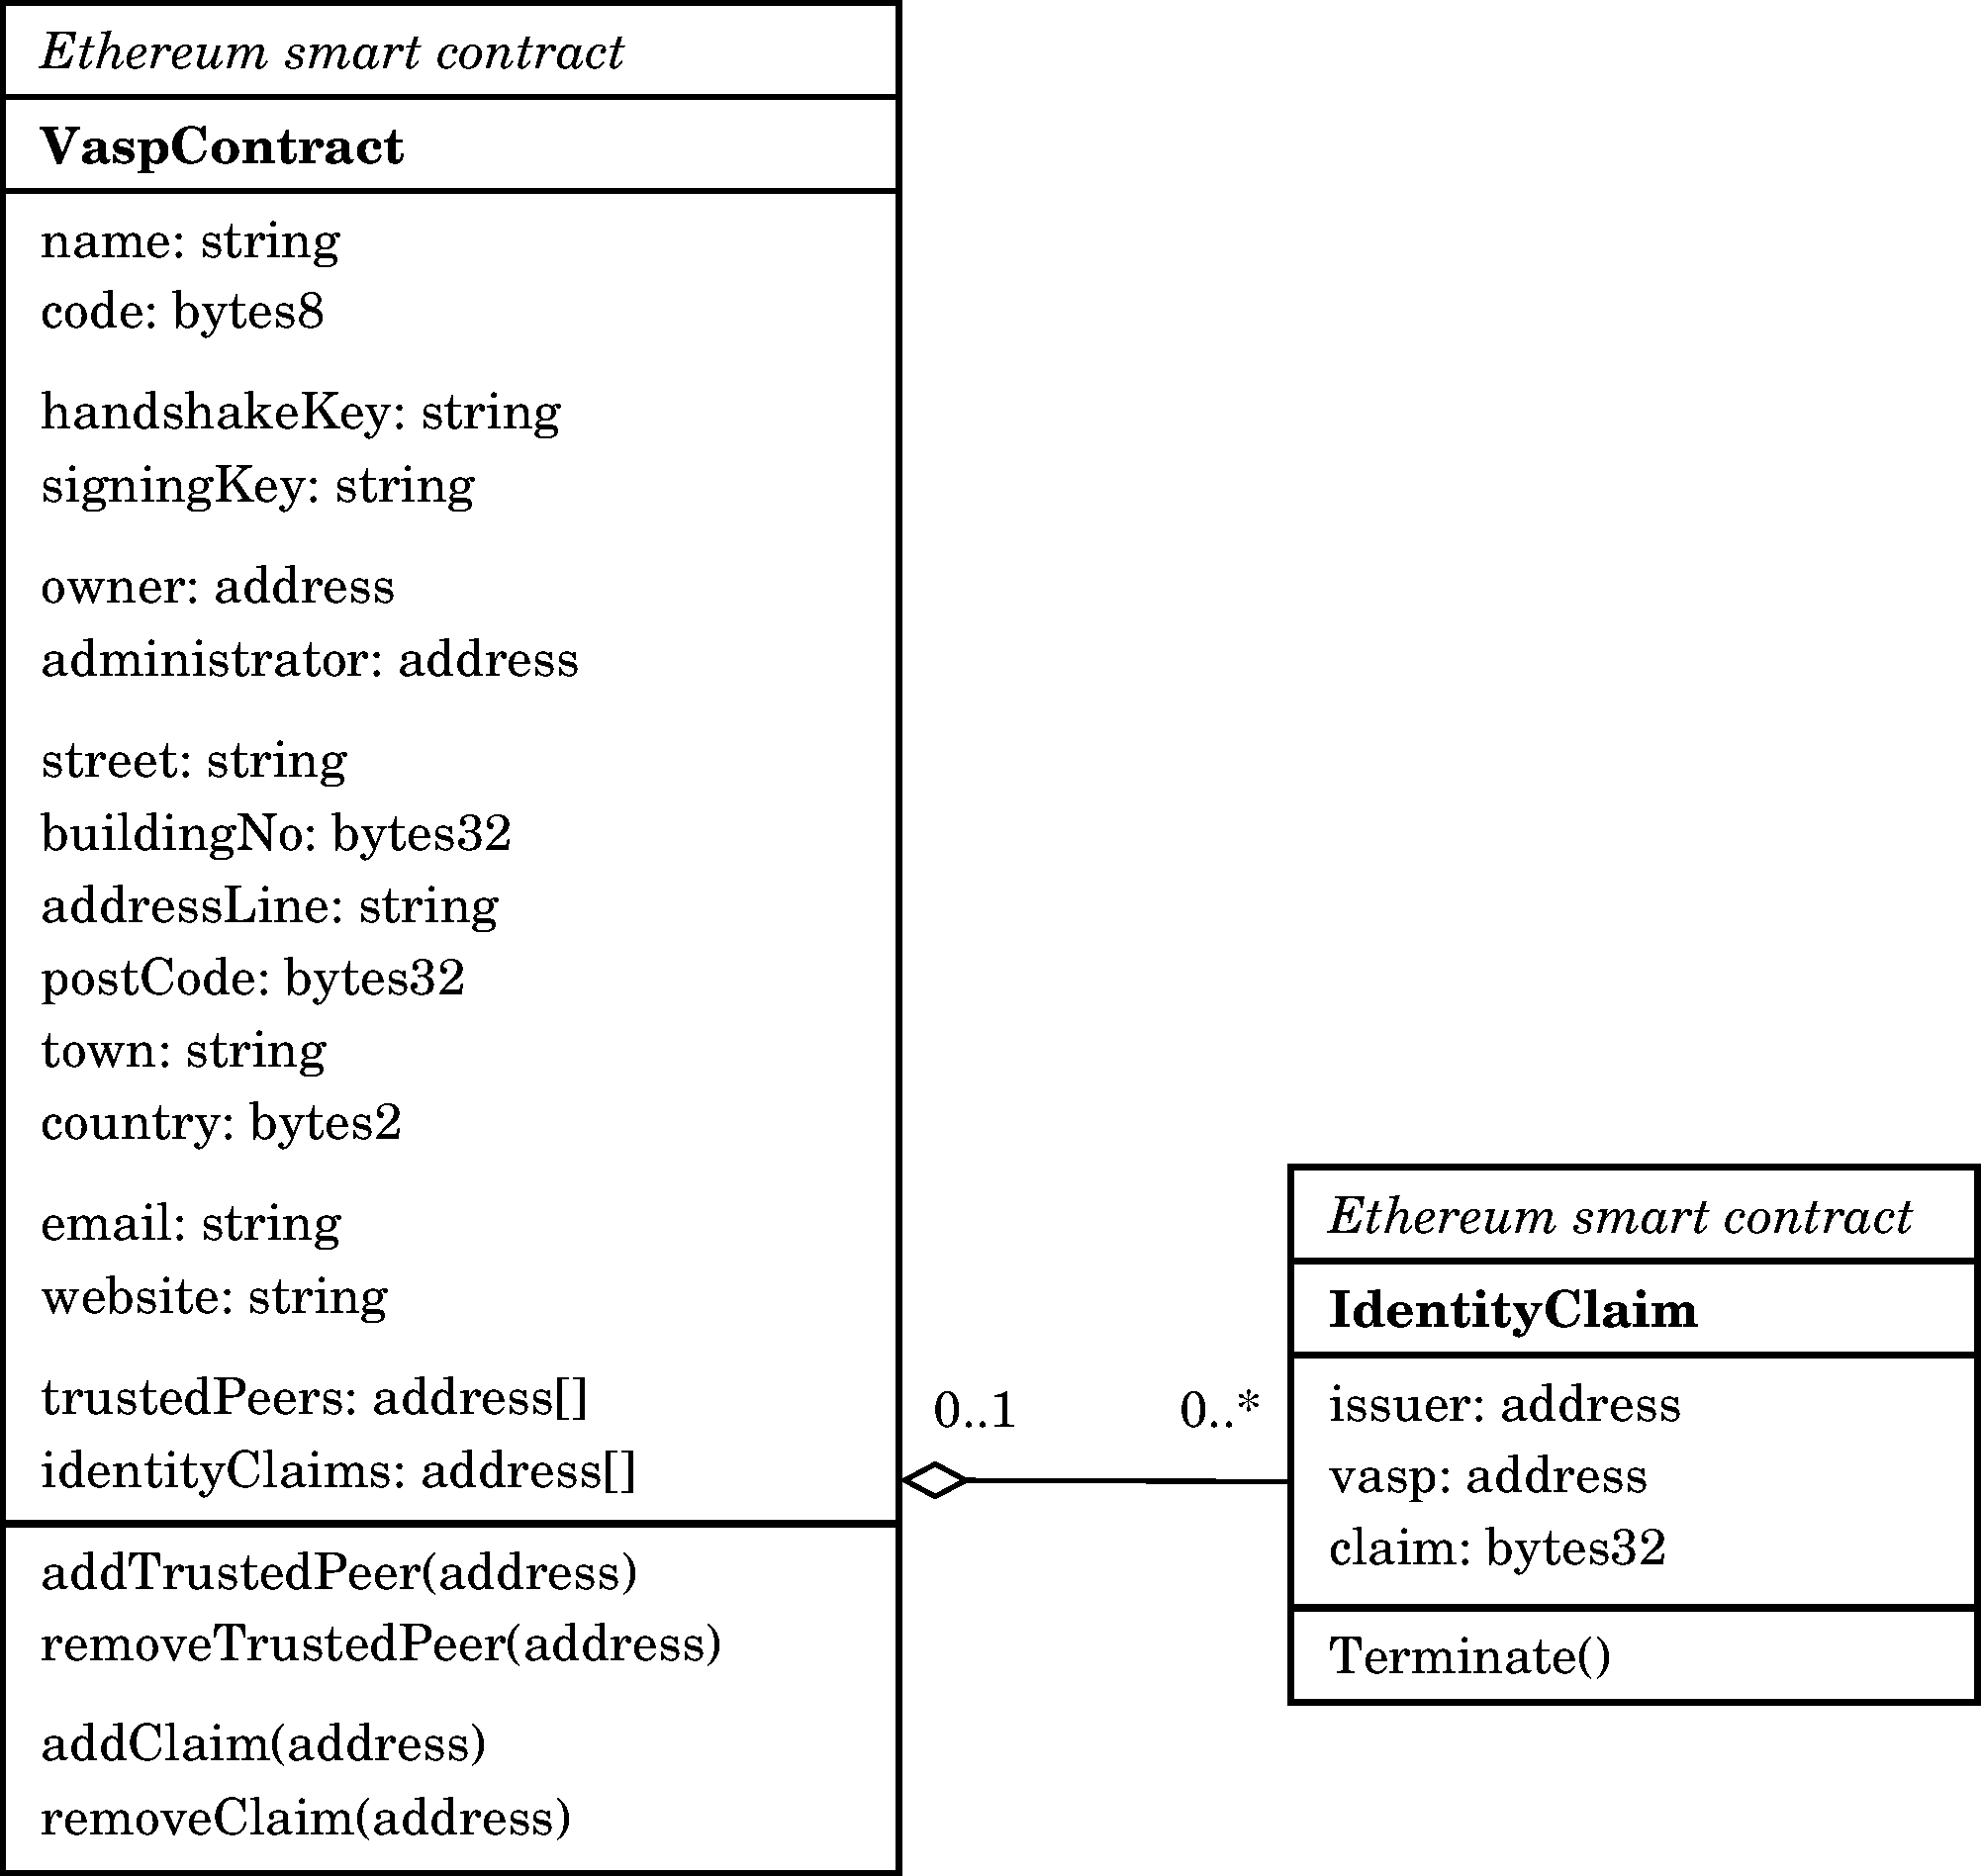
\includegraphics[width=0.8\textwidth]{g6.pdf}
\end{figure}

\subsubsection{VASP contract attributes (selection)}

\begin{tabular}{ l l }
\verb+name+&Legal name of the VASP\\[1ex]
\verb+code+&Last 32 bit of VASP contract address,\\
    &used as abbreviation for VASP identity\\[1ex]
\verb+channels+&Communication channels accepted by VASP for messages\\
    &(e.g. Whisper, Email, etc.)\\[1ex]
\verb+handshakeKey+&Asymmetric public key used to securely establish sessions\\[1ex]
\verb+signingKey+&Asymmetric public key used to verify message signatures\\[1ex]
\verb+owner+&Address assigned as the owner for the VASP contract\\[1ex]
\verb+administrator+&Address assigned to change smart contract attributes\\[1ex]
\verb+postal address+&Attributes for the VASP’s postal address, in line with section 7.10\\[1ex]
\verb+email, website+&Contact information\\[1ex]
\verb+trustedPeers+&Trusted peer VASPs\\[1ex]
\verb+identityClaims+&Identity claims made by trusted issuers\\[1ex]
\end{tabular}

\subsubsection{VASP contract methods (selection)}

\begin{tabular}{ l l }

\verb+addTrustedPeer(address)+&Adds peer VASP to the set of trusted peers.\\
    &Must be called by the administrator.\\[1ex]
\verb+removeTrustedPeer(address)+&Removes peer VASP from the set of trusted peers.\\
    &Must be called by the administrator.\\[1ex]
\verb+addClaim(address)+&Adds address of an identity claim contract, issued\\
    &by a trusted third party, to the set of accepted claims.\\ 
    &Must be called by the administrator.\\[1ex]
\verb+removeClaim(address)+&Removes address of an identity claim contract\\
    &from the set of accepted claims.\\
    &Must be called by the administrator.\\[1ex]

\end{tabular}

\subsection{Claim contract}

While mutual trust between VASPs can easily be recorded by reciprocal entries in their VASP contracts, identity claims made by third party issuers require a different setup. We propose the usage of a simple claim contract as part of the OpenVASP protocol.

Deployed by the issuer, the claim contract allows to specify the content and potential qualifications of the claim made about the VASP. Since the contract remains under control of the issuer, it can be revoked (terminated) at any time.

VASPs accept a claim made about them by adding the respective claim contract address. If for whatever reason necessary, claims can be repudiated by again removing the reference.

\subsection{Registering the VASP code in the Ethereum Name Service (ENS)}

The Ethereum Name Service (ENS) allows to use short, human-readable names as pointers to otherwise long Ethereum addresses. Its logic and governance are completely decentralized, operating solely as a set of smart contracts. The reader can find more information under https://ens.domains/.

As described in chapter 4, the VASP code is an abbreviation of the VASP contract address (VASP identity) and serves as prefix in the proposed VAAN format. Alternatively, the full contract address could have been used to uniquely bind a VAAN to the VASP identity on the blockchain. Using the shorter VASP code is obviously more convenient for everyday handling. However, it introduces the risk that an imposter could try to set up a smart contract with the same abbreviation as an existing VASP. Other VASPs may then be deceived into interacting with the wrong counterparty.

In order to mitigate this risk, VASPs must register their VASP code as an ENS domain and point it to their VASP contract. Taking the example from section 4.1, the VASP would register bb428798.eth and point it to the address \verb+0x7e7aeffa3a54d41929577873c47cbda7bb428798+.

The probability for a new VASP contract address to be the same as an existing one, is relatively low with one in $4.29 \times 109$. Nevertheless, if a collision was to happen, it would immediately be detected as the corresponding ENS domain would no longer be available for registration. In such as case, a simple redeployment of the contract generates a new contract address.

Besides providing security against imposters and accidental collisions, using the VASP code as ENS domain brings convenience as any VASP’s identity can be quickly retrieved by the 8-character code.

\subsection{Communication channels offered}

As described in chapter 3, different communication channels might be used to exchange protocol messages, and each VASP could decide which cannels to offer. Available options can be retrieved from the \textit{channels} attribute of the VASP contract.

\subsection{Summary: Steps to authenticate a VASP}

Whenever a counterparty VASP must be authenticated for the first time, the following steps are required to verify that a valid VASP identity is available.

\renewcommand{\theenumi}{\arabic{enumi}}
\begin{enumerate}
    \item Check if the 8-character VASP code, followed by the .eth domain suffix, resolves to the VASP contract address.
    \item Check if the standardized VASP contract was deployed and used as VASP identity.
    \item Check whether key attributes are properly filled out in the VASP contract.
    \item Check which of the VASPs listed as trusted peers in the VASP contract have reciprocally listed the counterparty VASP as a trusted peer.
    \item Review available identity claims issued by trusted third parties and verify their authenticity (e.g. by checking whether the known third party public address was used to set up the identity claim contract).
\end{enumerate}

Steps 1. to 3. are formal requirements and must be concluded with a positive result.

Information obtained in steps 4. and 5. require an assessment whether claims made by trusted peers and third parties is deemed to be sufficient for indirect authentication. If this is not the case, the VASP must be directly authenticated by obtaining first-hand evidence that the identity is genuine, e.g. by confirming the VASP identity via personal contact.

The above mentioned steps can largely be automated with exception of the final decision whether indirect authentication is enough to proceed.
\newpage


\section{Protocol Flow}

The protocol provides a set of requests and responses to facilitate a structured communication between the originator VASP and the beneficiary VASP transferring virtual assets on behalf of their respective customers.

At the outset, the beneficiary wants to receive virtual assets on a wallet hosted by the beneficiary VASP and therefore provides the originator with routing information on where to send them. The originator then instructs the originator VASP to transfer the virtual assets.

In the initiation phase, the involved VASPs establish communication and mutually authenticate and authorize each other. In transfer phase, originator/beneficiary information is exchanged, the transfer gets mutually approved and execution on the blockchain is notified and confirmed.

\begin{figure}[h]
    \centering
    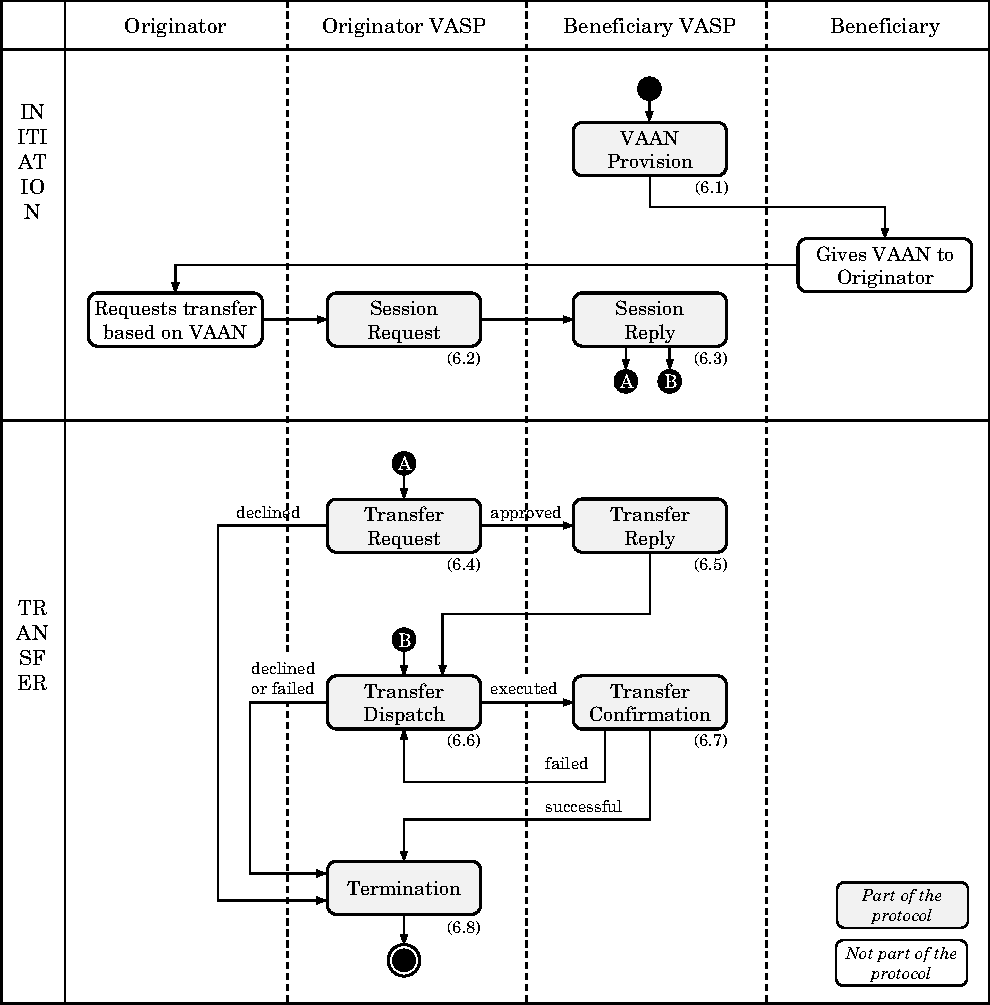
\includegraphics[width=\textwidth]{g7.pdf}
\end{figure}
\newpage

For the transfer phase, the protocol supports two different policies how a beneficiary VASP accepts virtual assets on behalf of their customers:
\renewcommand{\theenumi}{\alph{enumi}}
\begin{enumerate}
    \item \textbf{Approval required before blockchain transaction}\\
    Given the compliance obligations, the beneficiary VASP will generally want to approve a virtual asset transfer based on originator and beneficiary information before the actual blockchain transaction is executed. In addition, the beneficiary VASP can specify the destination address on the blockchain to be used for this transfer.
    \item \textbf{Approval NOT required before blockchain transaction}\\
    For efficiency reasons the VASPS may have agreed that an approval before the actual blockchain transaction is not required for certain transfers (e.g. transfers between two specific customers). As no message is exchanged before the blockchain transaction, either always the same destination address is used, or the originator VASP knows the destination address from a different source (e.g. using deterministic addresses based on a shared master public key). Such a practice can make sense when the VASPs regularly process numerous transactions for the same originator and beneficiary, e.g. as part of an automated setup.
\end{enumerate}

The following sections provide more details about each of the protocol steps.

\subsection{VAAN Provision}
\subsubsection{Processing steps by the beneficiary VASP}
\begin{figure}[h]
    \centering
    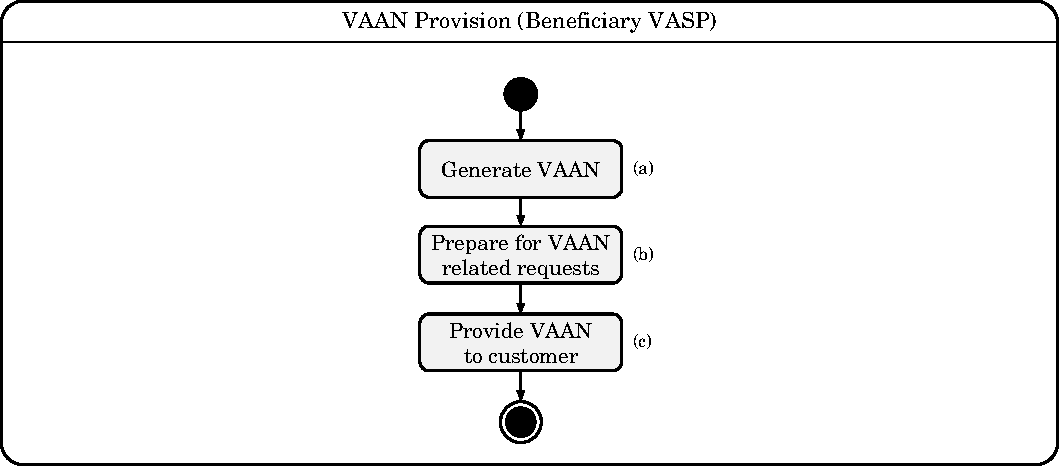
\includegraphics[width=0.8\textwidth]{g8.pdf}
\end{figure}
\begin{enumerate}
    \item Generate a customer specific VAAN based on the steps described in section 4.2.
    \item Ensure that incoming messages containing the VASP code as header can be received and processed (e.g. that the Whisper node is set up) and prepare internal systems and procedures to receive and process protocol messages related to the VAAN generated in the previous step.
    \item Provide the VAAN to the customer who can use it as routing information to receive virtual assets to the hosted wallet.
\end{enumerate}

\subsection{Session Request}
\begin{figure}[h]
    \centering
    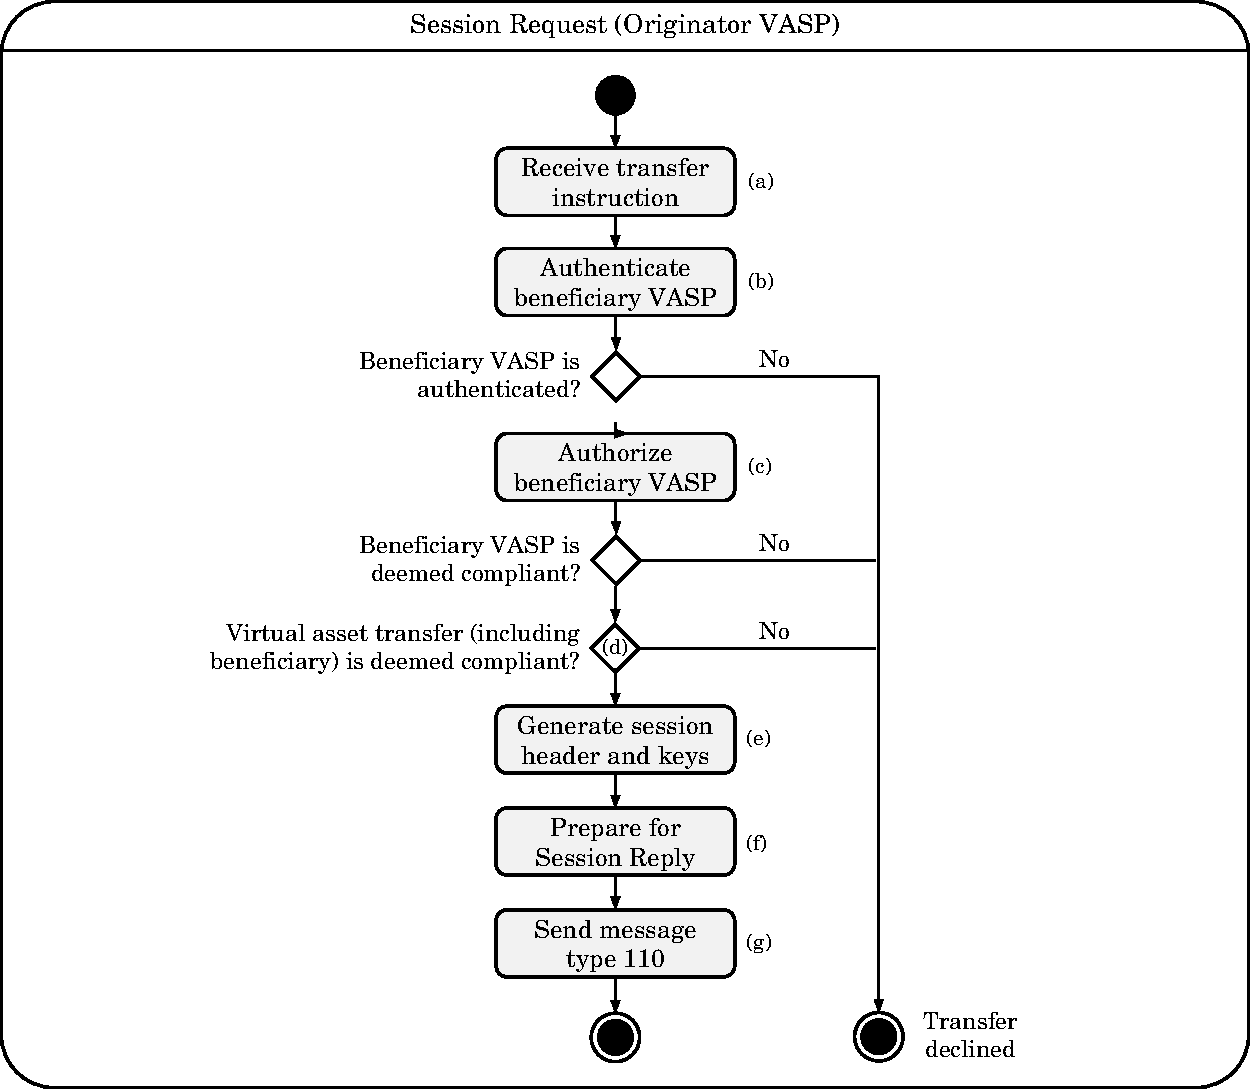
\includegraphics[width=\textwidth]{g9.pdf}
\end{figure}
\subsubsection{Processing steps by the originator VASP}
\begin{enumerate}
    \item Receive instruction from customer to transfer virtual asset to a wallet hosted with another VASP, specified by name and VAAN (see section 4.2) of the beneficiary.
    \item Identify and authenticate beneficiary VASP specified in the VAAN. See section 6.9 for authentication steps.
    \item Once successfully authenticated, authorize the beneficiary VASP (see section 6.10).
    \item Perform a risk-based decision whether a virtual asset transfer can be executed, based on all relevant information including information about the originator, the beneficiary, the beneficiary VASP, the virtual asset type and the amount of the requested transfer.
    \item Generate a random header (topic A) to be used in this session. Generate private and public keys based on the elliptic curve Diffie–Hellman (ECDH) key-exchange protocol to use for ephemeral encryption in transfer phase. Derive shared key based on the ECDH public key from the beneficiary VASP (handshakeKey in VASP contract) and own ECDH public key generated in the previous step.
    \item Prepare systems to receive the VARC Reply message from the beneficiary VASP (e.g. in the Whisper node, subscribe to messages with topic A and being encrypted with the shared key).
    \item Send Session Request message (type 110, see section 7.3) to the beneficiary VASP.
\end{enumerate}

\subsection{Session Reply}
\begin{figure}[h]
    \centering
    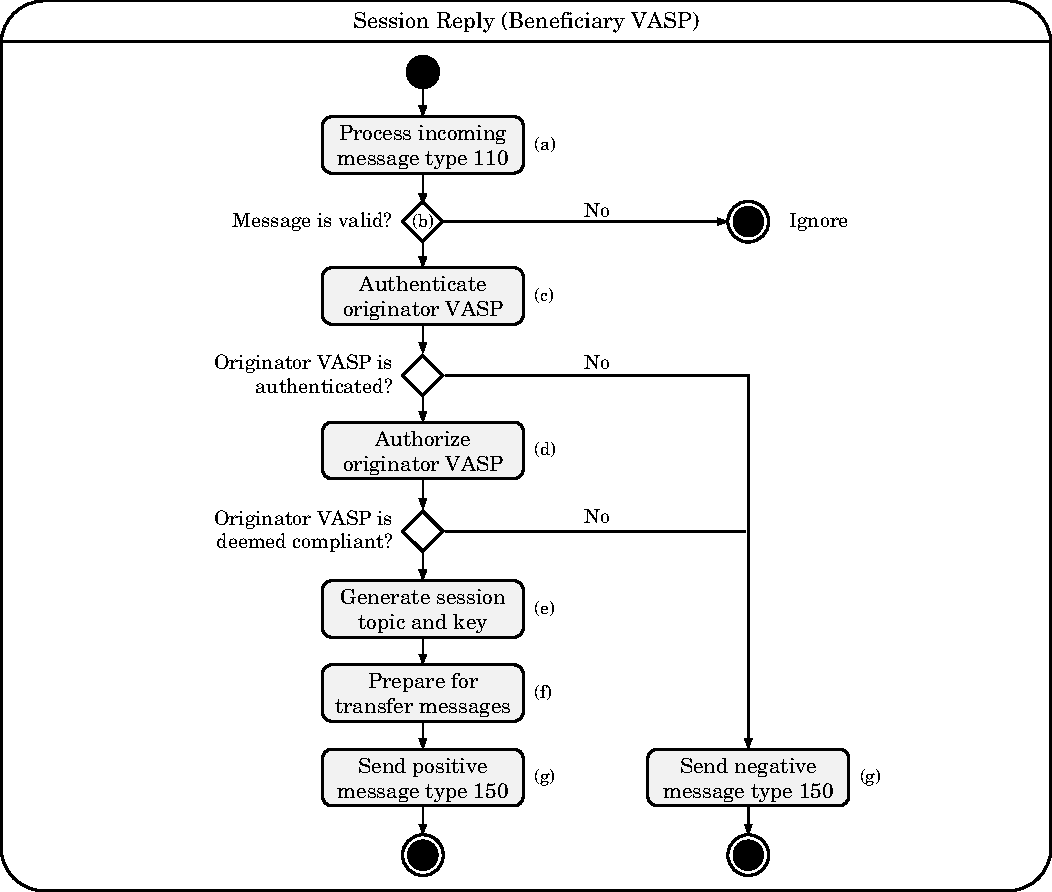
\includegraphics[width=\textwidth]{g10.pdf}
\end{figure}
\subsubsection{Processing steps by the beneficiary VASP}
\begin{enumerate}
    \item Receive Session Request message (type 110), e.g. from the Whisper node.
    \item Verify if incoming message contains mandatory data in valid format and is correctly signed.
    \item Authenticate the originator VASP. See section 6.9 for authentication steps.
    \item Once successfully authenticated, authorize the beneficiary VASP (see section 6.10).
    \item Generate a random header (topic B) to be used in this session. Derive shared key based on the ECDH public key from the originator VASP (received in message) and own ECDH public key.
    \item Prepare systems to receive subsequent messages from the originator VASP (e.g. in the Whisper node, subscribe to messages with topic B and being encrypted with the shared key).
    \item Send Session Reply message (type 150, see section 7.4) to the originator VASP. In case of failed authentication (step c) or failed authorization (step d), a negative message is sent by providing the response code specifying the reason for failure.
\end{enumerate}

\subsection{Transfer Request}
\subsubsection{Processing steps by the originator VASP}
\begin{figure}[h]
    \centering
    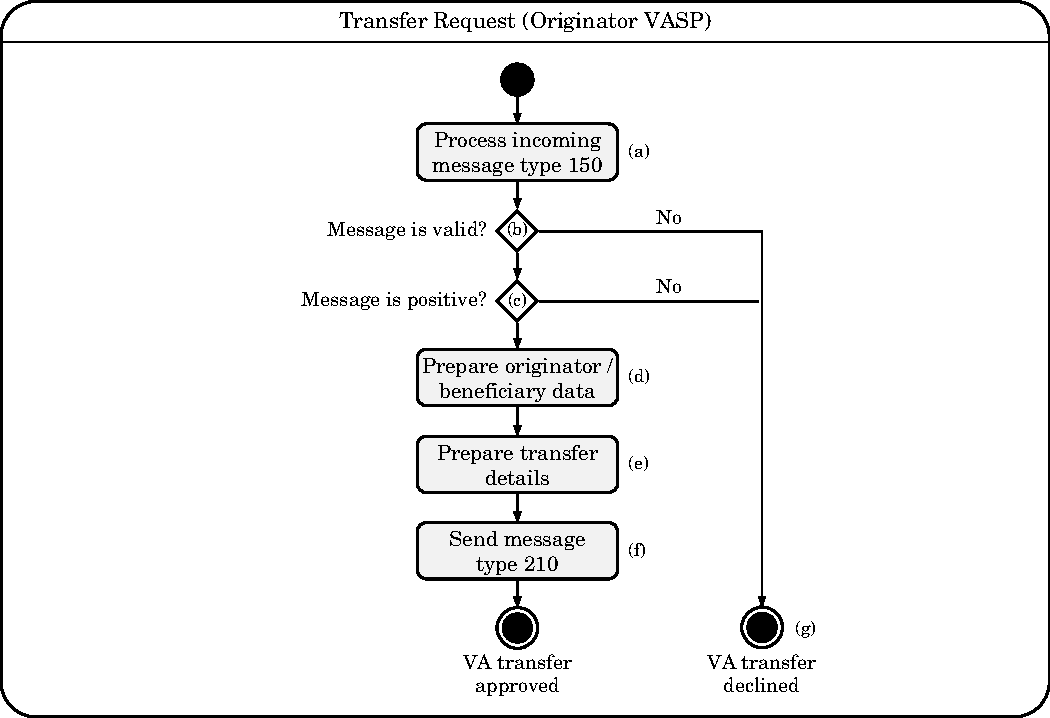
\includegraphics[width=\textwidth]{g11.pdf}
\end{figure}
\begin{enumerate}
    \item Receive Session Reply message (type 150), e.g. from the Whisper node.
    \item Verify if incoming message contains mandatory data in valid format and is correctly signed.
    \item Check whether received message has a positive response code.
    \item Prepare originator and beneficiary data (see sections 7.11 and 7.12 for details).
    \item Prepare transfer session details (virtual asset type, transfer type and amount).
    \item Send Transfer Request message (type 210, see section 7.5) to the beneficiary VASP.
    \item In case of an invalid or negative incoming message (steps b or c), the session is terminated following the steps in section 6.6.
\end{enumerate}


\subsection{Transfer Reply}
\subsubsection{Processing steps by the beneficiary VASP}
\begin{figure}[h]
    \centering
    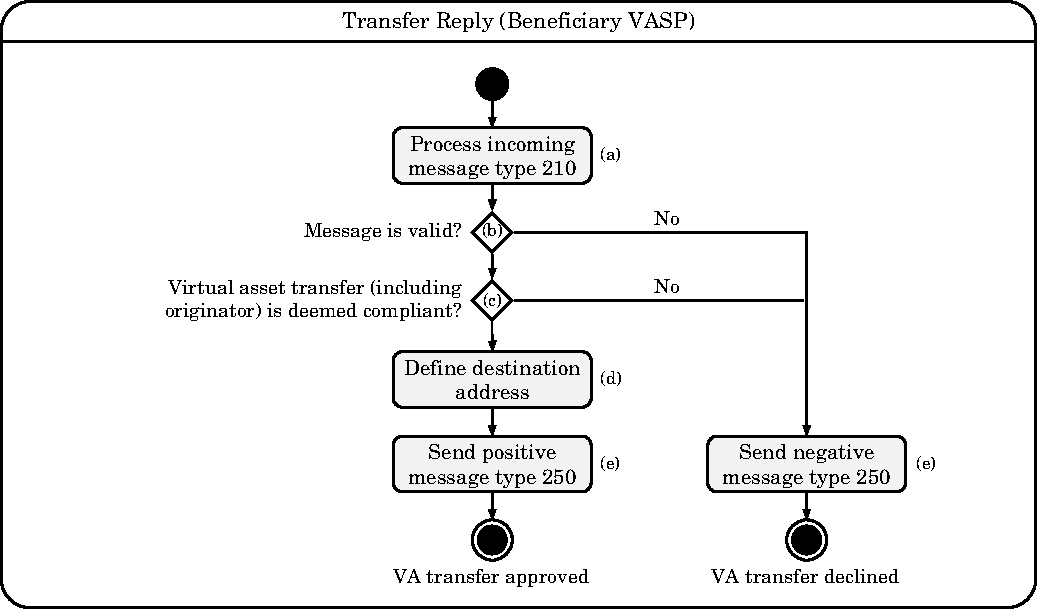
\includegraphics[width=\textwidth]{g12.pdf}
\end{figure}
\begin{enumerate}
    \item Receive Transfer Request message (type 210), e.g. from the Whisper node.
    \item Verify if incoming message contains mandatory data in valid format and is correctly signed.
    \item Perform a risk-based decision whether the requested virtual asset transfer can be executed, based on all relevant information including information about the originator, the beneficiary, the beneficiary VASP, the virtual asset type and the amount of the requested transfer.
    \item Define destination address to be used for the virtual asset transfer.
    \item Send Transfer Replay message (type 250, see section 7.6) to the originator VASP. In case of an invalid incoming message (step b) or if the transfer is deemed to be non-compliant, a negative message is sent by providing the response code specifying the reason for failure.
\end{enumerate}

\subsection{Transfer Dispatch}
\begin{figure}[h]
    \centering
    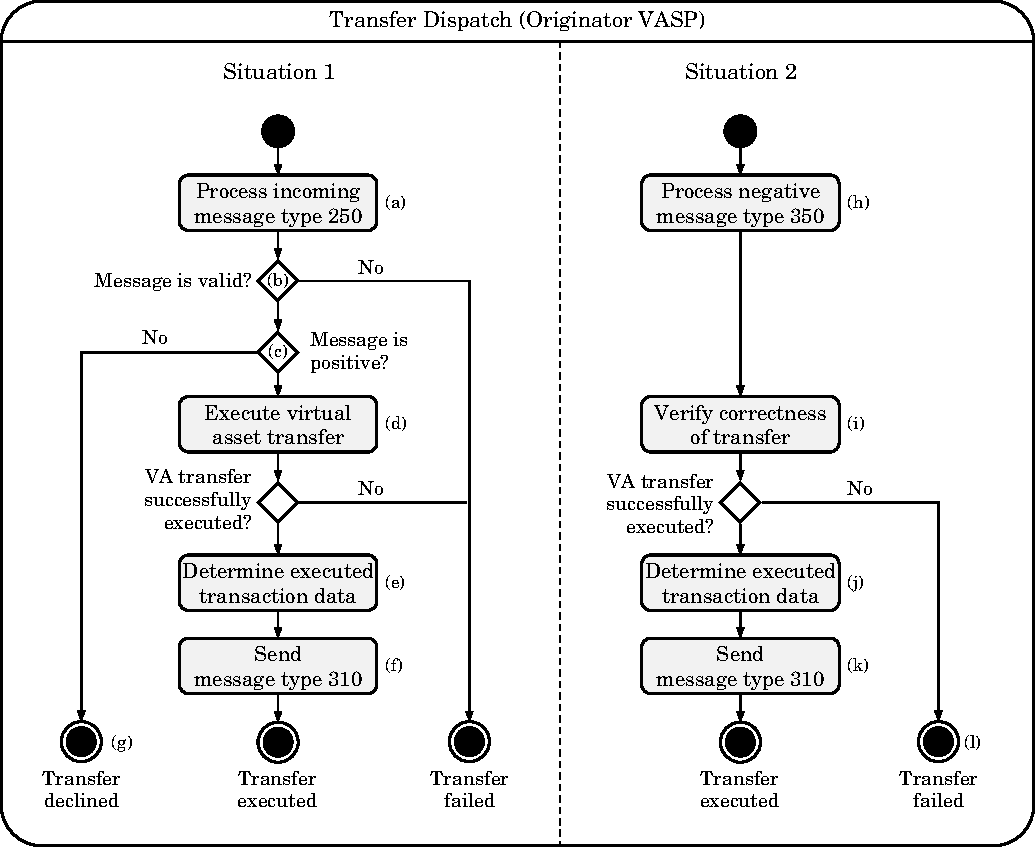
\includegraphics[width=\textwidth]{g13.pdf}
\end{figure}
\subsubsection{Processing steps by the originator VASP (situation 1)}
\begin{enumerate}
    \item Receive Transfer Reply message (type 250), e.g. from the Whisper node.
    \item Verify if incoming message contains mandatory data in valid format and is correctly signed.
    \item Check whether received message has a positive response code.
    \item Execute the virtual asset transfer by posting the transaction to the blockchain or distributed ledger technology (DLT) system. Check whether the transaction has been successfully executed, considering the specifics of the technology used for the transfer (e.g. awaiting a number of confirmations). Repeat if necessary.
    \item Determine transaction information (identifier, date and time of execution and sending address, if applicable).
    \item Send Transfer Dispatch message (type 310, see section 7.7) to the beneficiary VASP.
    \item In case of an invalid or negative incoming message (steps b or c) or if the transfer could not be executed (e.g. for technical reasons), a negative message is sent by providing the response code specifying the reason for failure.
\end{enumerate}

\subsubsection{Processing steps by the originator VASP (situation 2)}
\begin{enumerate}
    \item Receive negative Transfer Confirmation message (type 350), e.g. from the Whisper node.
    \item Verify whether transaction has been correctly executed and analyze the reason for negative confirmation from the beneficiary VASP. Repeat execution of transaction if necessary.
    \item Determine transaction information (identifier, date and time of execution and sending address, if applicable).
    \item Send new Transfer Dispatch message (type 310, see section 7.7) to the beneficiary VASP, specifying the result of the verification.
    \item If the transfer could (still) not be executed (e.g. for technical reasons), a negative message is sent with a response code specifying the reason for failure.
\end{enumerate}

\newpage
\subsection{Transfer Confirmation}
\begin{figure}[h]
    \centering
    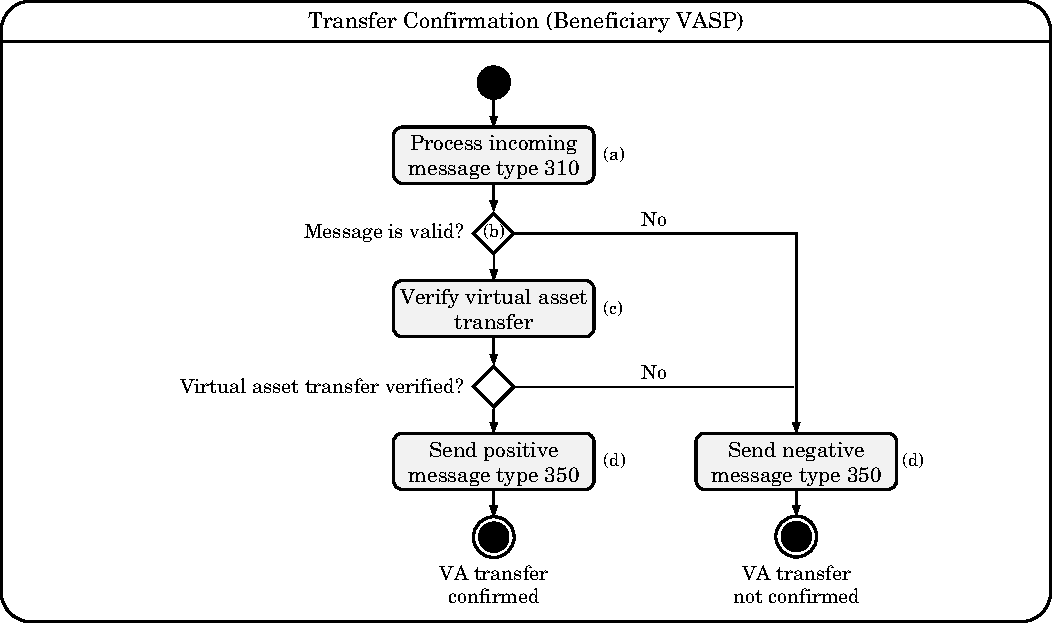
\includegraphics[width=\textwidth]{g14.pdf}
\end{figure}
\subsubsection{Processing steps by the beneficiary VASP}
\begin{enumerate}
    \item Receive Transfer Dispatch message (type 310), e.g. from the Whisper node.
    \item Verify if incoming message contains mandatory data in valid format and is correctly signed.
    \item Check whether the transaction has been successfully executed on the blockchain or distributed ledger technology (DLT) system, considering the specifics of the technology used for the transfer (e.g. awaiting a number of confirmations). Verify whether received transaction information is accurate.
    \item Send Transfer Confirmation message (type 350, see section 7.8) to the originator VASP. In case of an invalid incoming message (step b) or if the transaction has not been successfully executed or is not matching the transaction information received in message 310 (step c), a negative message is sent gy providing the response code specifying the reason for failure.
\end{enumerate}

\newpage
\subsection{Termination}
\begin{figure}[h]
    \centering
    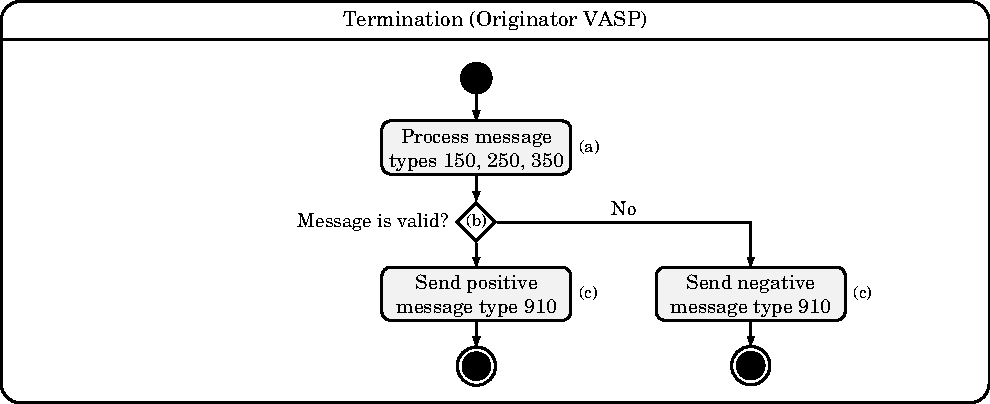
\includegraphics[width=\textwidth]{g15.pdf}
\end{figure}
\subsubsection{Processing steps by the originator VASP}
\begin{enumerate}
    \item Receive Session Reply (type 150),  Transfer Reply (type 250) or Transfer Confirmation (type 350) message, e.g. from the Whisper node.
    \item Verify if incoming message contains mandatory data in valid format and is correctly signed.
    \item Send Termination message (type 910, see section 7.8) to the originator VASP. In case of an invalid incoming message (step b) or if the transaction has not been successfully executed or is not matching the transaction information received in message 310 (step c), a negative message is sent by providing the response code specifying the reason for failure.
\end{enumerate}

\subsection{Authentication}
\begin{figure}[h]
    \centering
    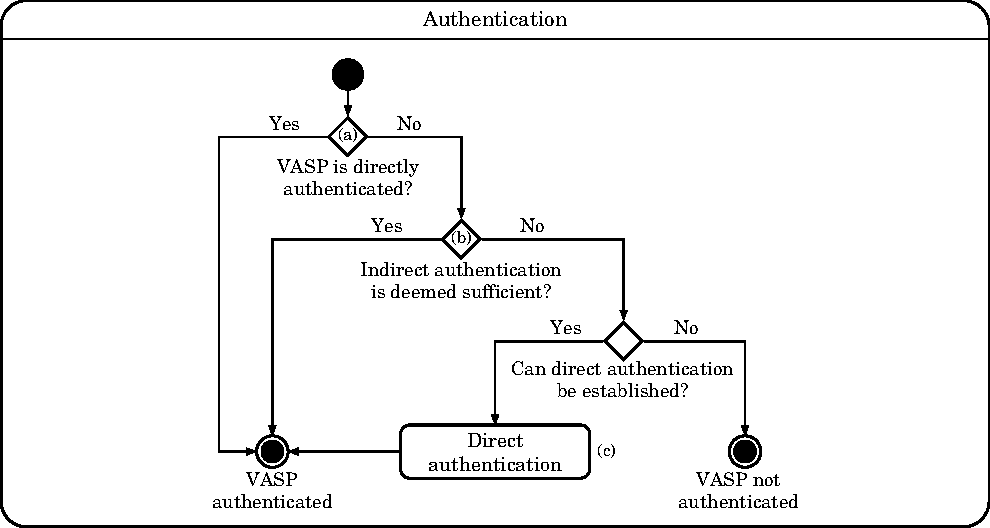
\includegraphics[width=0.8\textwidth]{g16.pdf}
\end{figure}
\subsubsection{Processing steps}
\begin{enumerate}
    \item Ideally, the receiving VASP can be directly authenticated, which means first-hand evidence that the identity is genuine (e.g. obtaining the VASP identity via personal contact).
    \item Indirect authentication can be achieved if both sending and receiving VASP share a web of trust involving other VASPs or by checking the counterparty’s identity claims issued by thrusted third parties.
    \item If indirect authentication is deemed not to be enough, establishing direct authentication should be considered.
\end{enumerate}
See chapter 5 for more details about authentication.


\subsection{Authorization}

\begin{figure}[h]
    \centering
    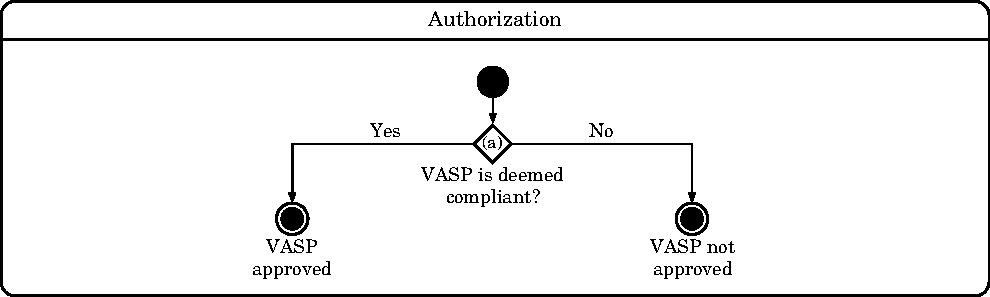
\includegraphics[width=\textwidth]{g17.pdf}
\end{figure}
\subsubsection{Processing steps}
\begin{enumerate}
    \item The VASP must evaluate whether the counterparty VASP is acceptable or not in order to comply with applicable laws and regulations.	Particularly the rules regarding anti-money laundering, sanctions and the combating the financing of terrorism must be applied when evaluating the counterparty VASP. Decision is taken following a risk-based approach and differs from VASP to VASP.
\end{enumerate}

Important: the decision whether a virtual asset transfer can be executed is not only based on the counterparty VASP, but primarily by analyzing originator and beneficiary information. This step is solely about the assessment on the counterparty VASP involved in the transfer once identified and authenticated.	
\newpage
\section{Protocol Messages}

\subsection{Message Types}
The protocol includes seven structured message types as summarized in the table below. Protocol messages are specified to use the JSON format, which is human-readable as well as common for data processing.

Each message contains relevant header information and is signed with the sender’s private key.  Certain content is deliberately repeated in the different messages to provide complete information about the virtual asset transfer in its respective state when looking at a specific message. In this way, messages can be directly filed and maintained in compliance with applicable regulations.

This set of message types is meant to form the basis for a more extended VASP-to-VASP protocol with additional message types to be included based on community requirements. Therefore, session initiation using message types 110 and 150 is designed to be a generic handshake for any message types to follow. Similarly, message type 910 is solely closing the session in the end.

One of the most obvious additions would be message types for bulk transfers of virtual assets, which might be particularly relevant for larger VASPs. However, it seems reasonable to first gain experience on single transfers first and expand the protocol based on the learnings of the user base.

Details for the seven message types can be found in sections 7.3 to 7.9 of this chapter.
\begin{figure}[h]
    \centering
    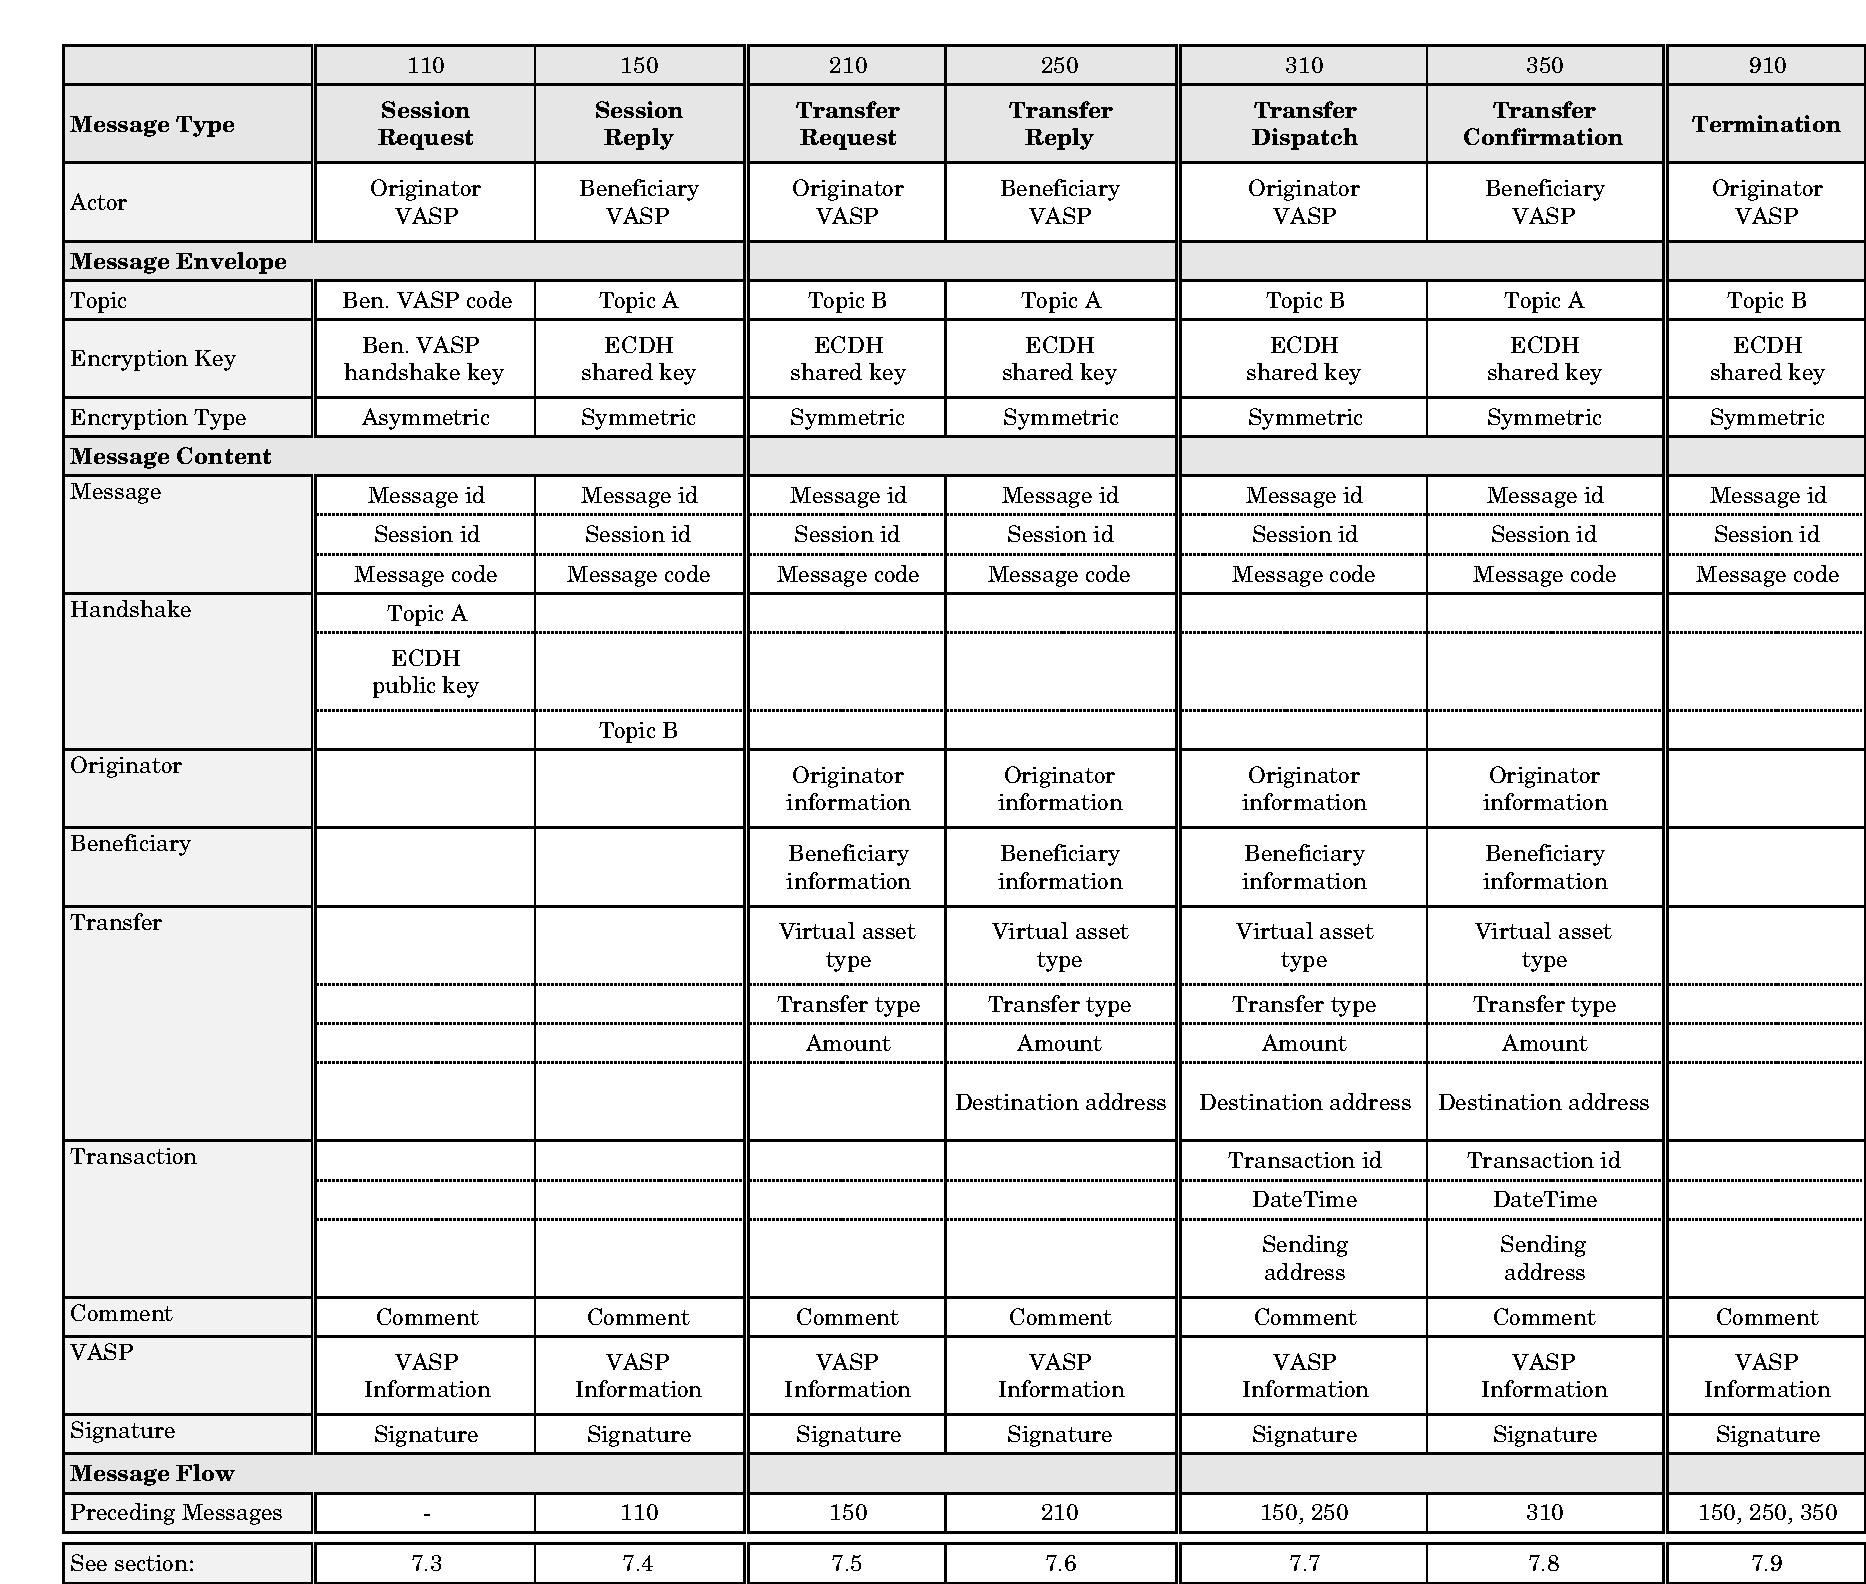
\includegraphics[width=0.9\textwidth]{g18.pdf}
\end{figure}

\subsection{Session Model}
All messages exchanged for a virtual asset transfer form a session. Sessions are initiated by message type 110 and acknowledged by message type 150.

The initiation phase includes the exchange of public keys to generate a shared symmetric key following the elliptic curve Diffie–Hellman (ECDH) protocol. In addition, both VASPs exchange random headers to be used for message routing in transfer phase (topic A and topic B).

Following initiation phase, originator and beneficiary information can be exchanged ensuring forward secrecy, as the long-term keys are used for authentication purposes only.
\begin{figure}[h]
    \centering
    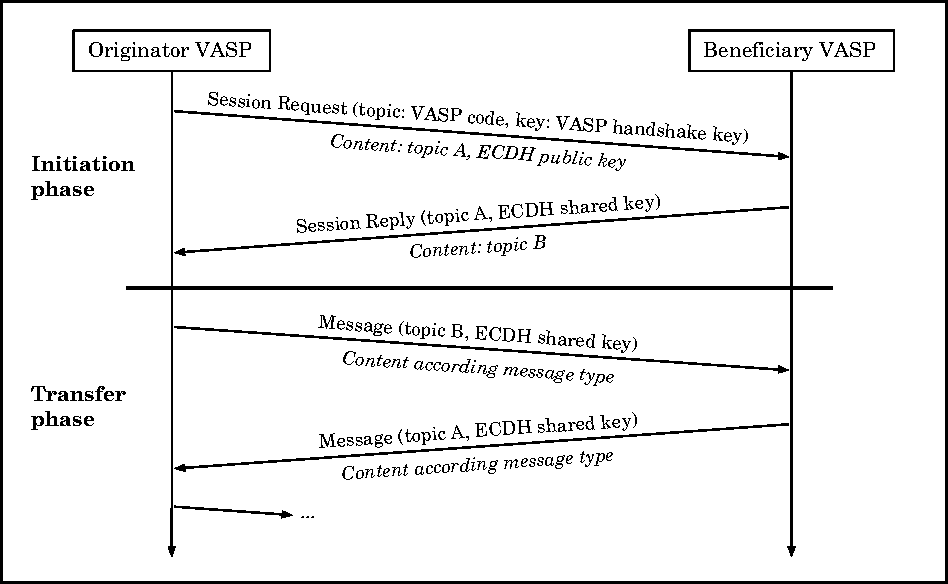
\includegraphics[width=\textwidth]{g19.pdf}
\end{figure}
\subsubsection{Encryption system and parameter selection}

Cryptographic algorithms used and all its parameter (e.g. key lengths) must be thoroughly challenged and carefully selected as part of the final protocol specification. The following suggestions are meant as a starting point for discussion:
\begin{enumerate}
    \item \textbf{Session request message:}\\
    Asymmetric encryption SECP-256k1 as per Whisper standard, using the handshakeKey published in the VASP contract (see section 5.2).
    \item \textbf{All other messages:}\\
    Symmetric encryption with the AES GCM algorithm as per Whisper standard, 256-bit key with random 96-bit nonce.
\end{enumerate}
Shared key generated via the X25519 key exchange protocol with a fixed key length of 256 bit. Salting as well as an appropriate key derivation function must be defined, considering that one of the two public ECDH keys is published in the VASP contract and therefore reused.

\subsection{Session Request}
\subsubsection{Message purpose}
Initiates a session between two VASPs. First part of a two-way handshake between VASPs to finally generate a shared symmetric session key based on the Diffie–Hellman key-exchange protocol

\subsubsection{Message structure}
\begin{figure}[h]
    \centering
    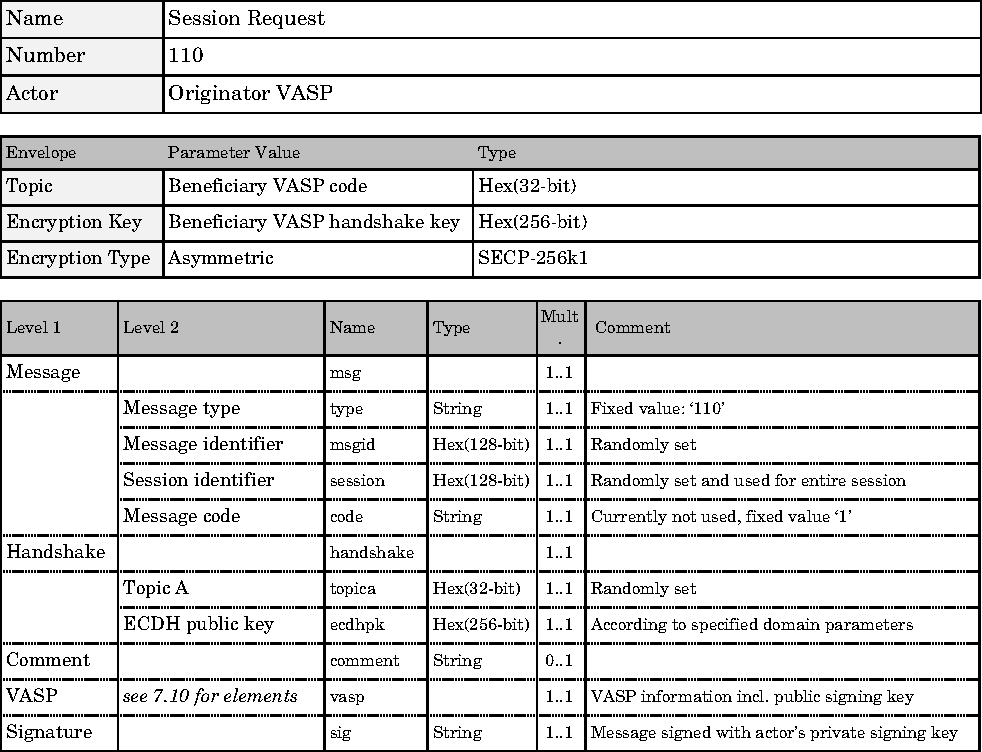
\includegraphics[width=\textwidth]{g20.pdf}
\end{figure}
\newpage



\subsection{Session Reply}
\subsubsection{Message purpose}
Response (positive or negative) to a previous request for initiating a session between two VASPs. Second part of a two-way handshake.


\subsubsection{Message structure}
\begin{figure}[h]
    \centering
    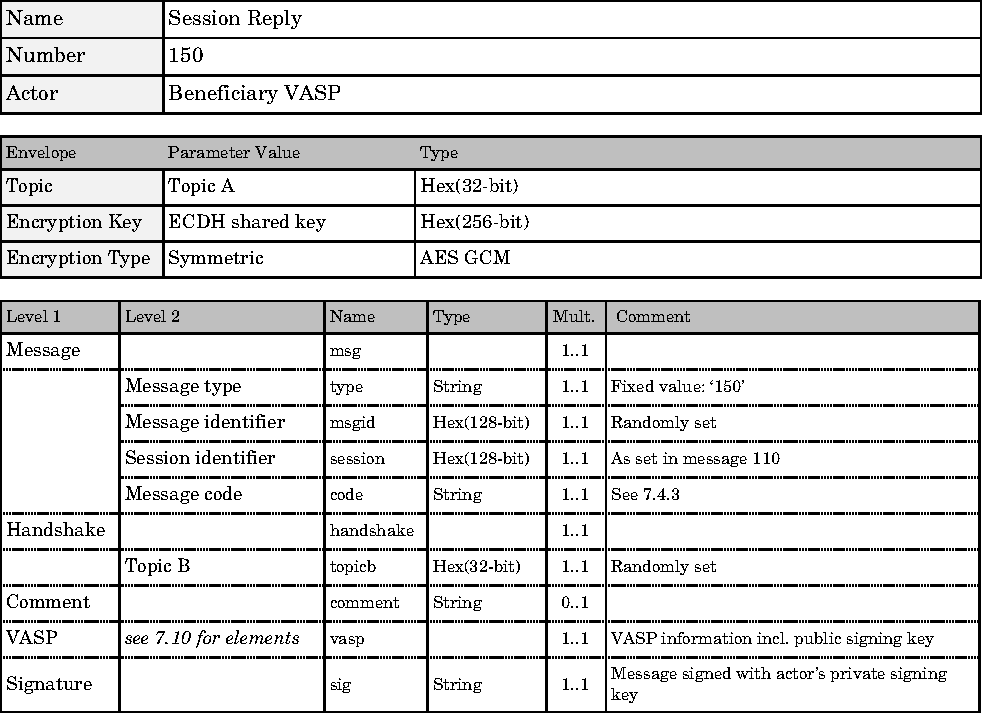
\includegraphics[width=\textwidth]{g21.pdf}
\end{figure}
\subsubsection{Possible message codes}
\verb+1+ = Session accepted\\
\verb+2+ = Session declined; request not valid\\
\verb+3+ = Session declined; originator VASP could not be authenticated\\
\verb+4+ = Session declined; originator VASP declined\\
\verb+5+ = Session declined; temporary disruption of service\\
\newpage

\subsection{Transfer Request}
\subsubsection{Message purpose}
Seeking approval from the beneficiary VASP for a virtual asset transfer by specifying transfer details including originator and beneficiary information.
\subsubsection{Message structure}
\begin{figure}[h]
    \centering
    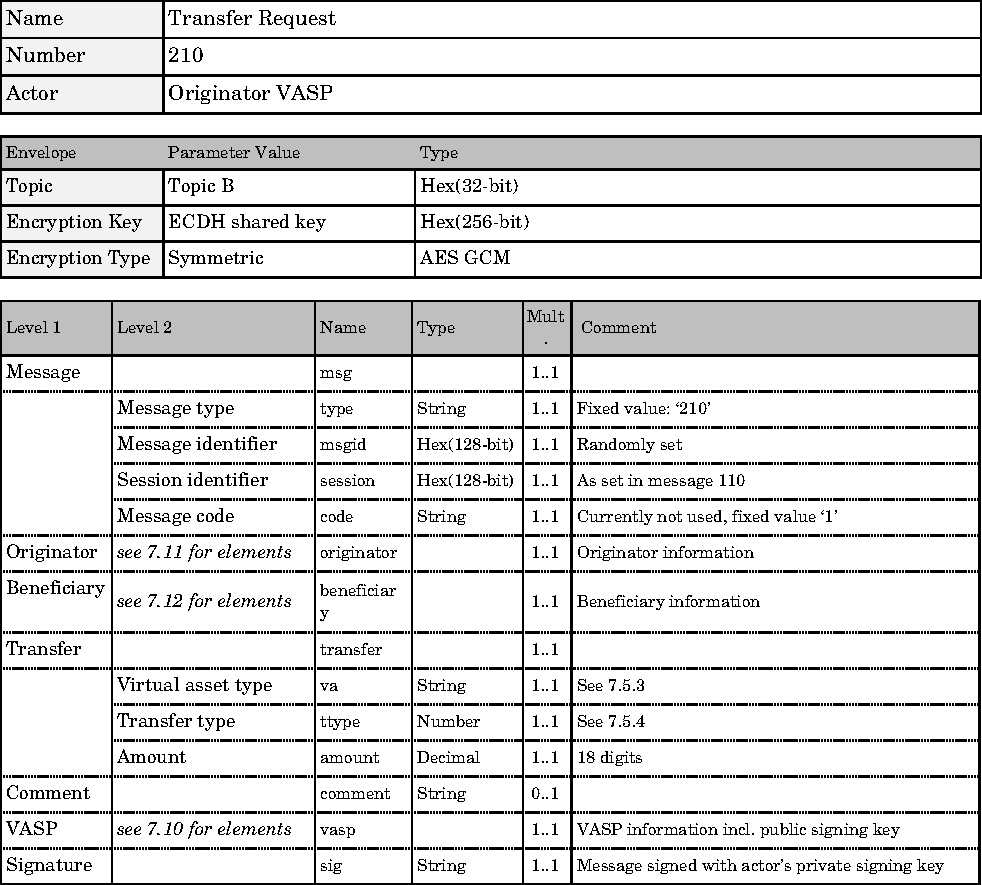
\includegraphics[width=\textwidth]{g22.pdf}
\end{figure}
\subsubsection{Possible transfer types}
Examples: \verb+BTC+ = Bitcoin, \verb+ETH+ = Ethereum.
To be defined as part of community governance.
\subsubsection{Possible transfer types}
\verb+1+ = Blockchain transaction (no further codes defined at the moment, but used to specify alternative transfer types, e.g. Layer 2 mechanisms)
\newpage

\subsection{Transfer Reply}
\subsubsection{Message purpose}
Response (positive or negative) to an originator VASP having sought approval for a virtual asset transfer by specifying transfer details including originator and beneficiary information.
\vspace{-1em}
\subsubsection{Message structure}
\vspace{-1em}
\begin{figure}[h]
    \centering
    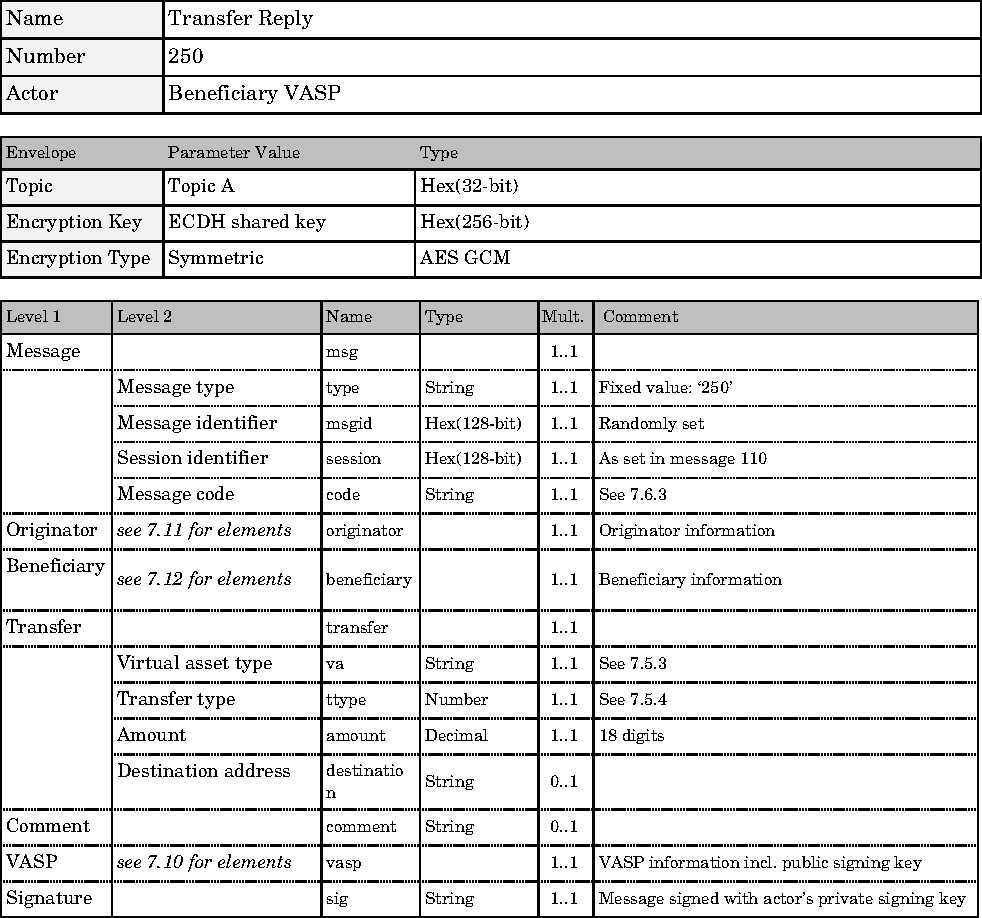
\includegraphics[width=\textwidth]{g23.pdf}
\end{figure}
\subsubsection{Possible message codes}
\verb+1+ = Transfer accepted\\
\verb+2+ = Transfer declined; request not valid\\
\verb+3+ = Transfer declined; no such beneficiary\\
\verb+4+ = Transfer declined; virtual asset not supported\\
\verb+5+ = Transfer declined; transfer not authorized\\
\verb+6+ = Transfer declined; temporary disruption of service\\
\newpage


\subsection{Transfer Dispatch}
\subsubsection{Message purpose}
Notifies the beneficiary VASP that a virtual asset transaction has been committed to the blockchain.
\subsubsection{Message structure}
\begin{figure}[h]
    \centering
    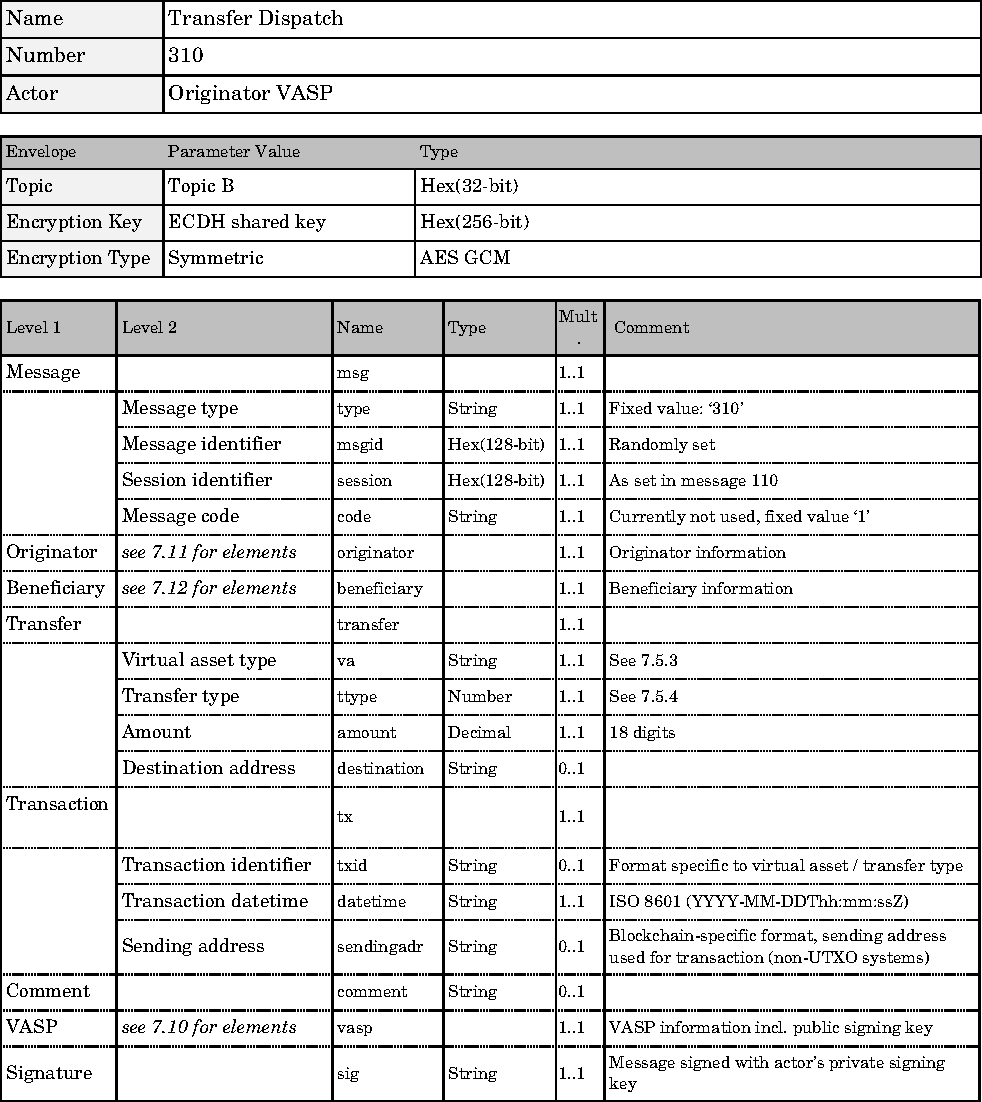
\includegraphics[width=\textwidth]{g24.pdf}
\end{figure}
\subsection{Transfer Confirmation}
\subsubsection{Message purpose}
Positive or negative acknowledgement to the originator VASP about the receipt of virtual assets transferred via a blockchain transaction.
\subsubsection{Message structure}
\begin{figure}[h]
    \centering
    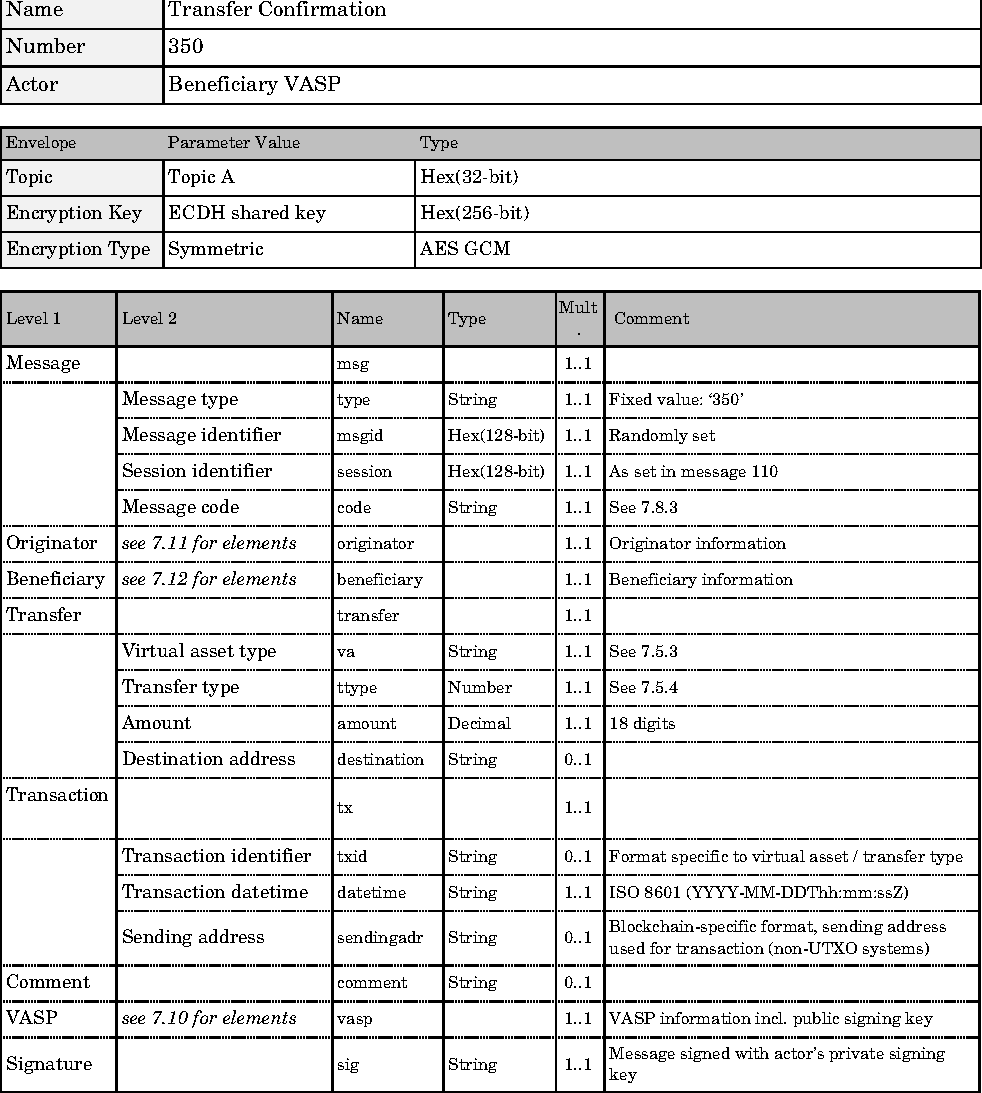
\includegraphics[width=\textwidth]{g25.pdf}
\end{figure}
\subsubsection{Possible message codes}
\verb+1+ = Transfer accepted\\
\verb+2+ = Transfer declined; dispatch not valid\\
\verb+3+ = Transfer declined; assets not received\\
\verb+4+ = Transfer declined; wrong amount\\
\verb+5+ = Transfer declined; wrong asset\\
\verb+6+ = Transfer declined; transaction data mismatch\\
\newpage

\subsection{Termination}
\subsubsection{Message purpose}
Terminates a session between two VASPs.

\subsubsection{Message structure}
\begin{figure}[h]
    \centering
    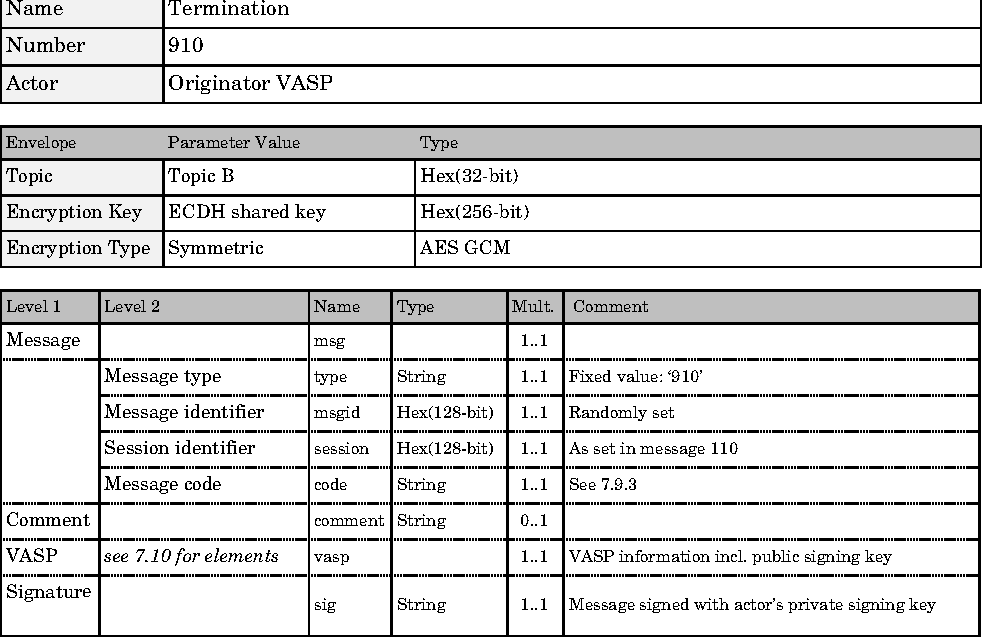
\includegraphics[width=\textwidth]{g26.pdf}
\end{figure}
\subsubsection{Possible message codes}
\verb+1+ = Session closed; transfer occurred\\
\verb+2+ = Session closed; transfer declined by beneficiary VASP\\
\verb+3+ = Session closed; transfer canceled by originator VASP\\
\newpage


\subsection{VASP Information}
Mandatory and optional elements for transmitting information about the VASPs involved in the virtual asset transfer.
\begin{figure}[h]
    \centering
    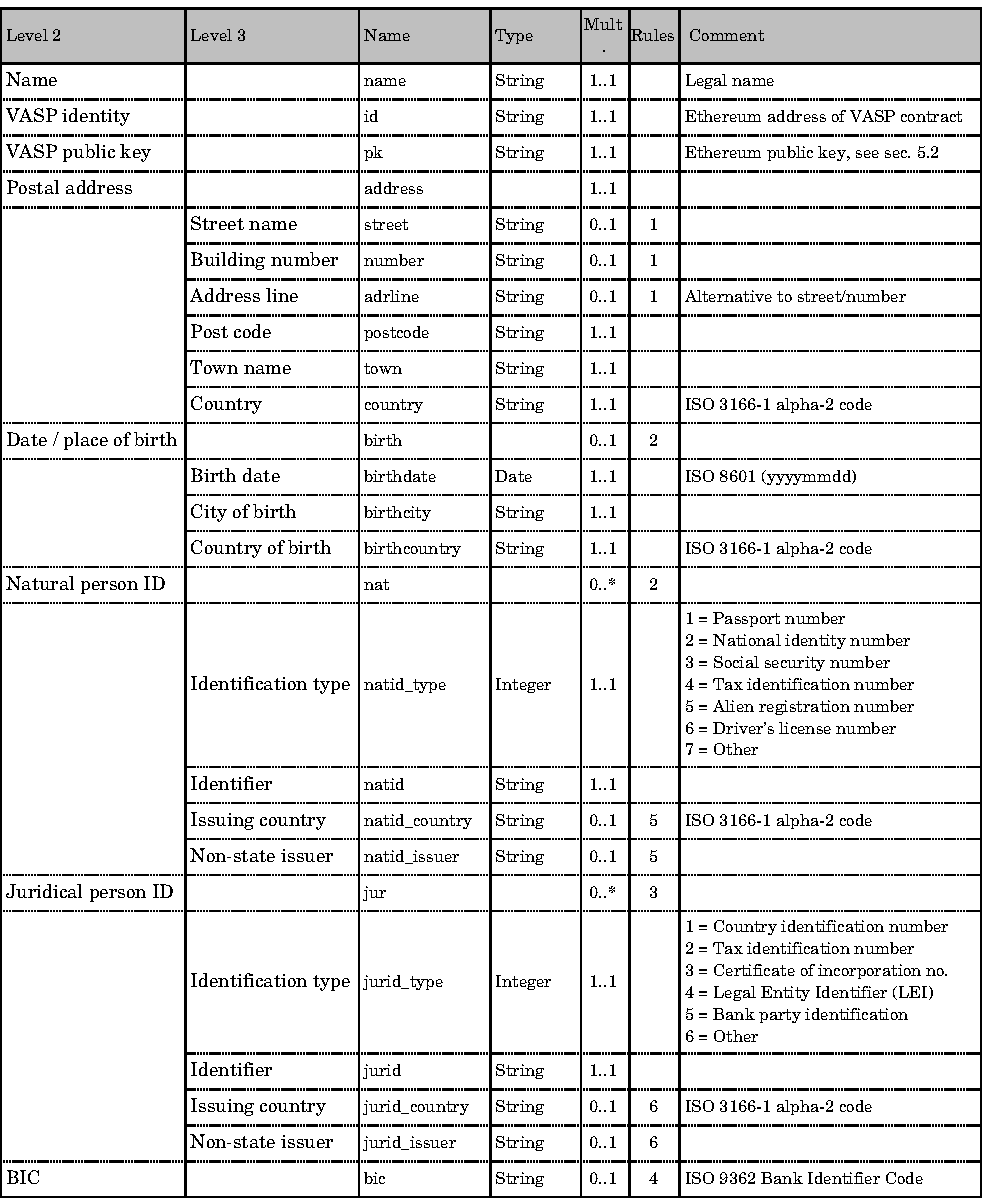
\includegraphics[width=\textwidth]{g27.pdf}
\end{figure}
\newpage

\subsubsection{Rules}
\renewcommand{\theenumi}{\arabic{enumi}}
\begin{enumerate}
\item Either \verb+[street]+ and \verb+[number]+ must both be present or \verb+[adrline]+. All three positions can be present at the same time.
\item \verb+[birth]+ or \verb+[nat]+ is allowed, if neither \verb+[jur]+ nor \verb+[bic]+ is present.
\item \verb+[jur]+ is allowed, if neither \verb+[birth]+ nor \verb+[nat]+ nor \verb+[bic]+ is present.
\item \verb+[bic]+ is allowed, if neither \verb+[birth]+ nor \verb+[nat]+ nor \verb+[jur]+ is present.
\item If \verb+[nat]+ is present, either \verb+[natid_country]+ or \verb+[natid_issuer]+ or both must be present.
\item If \verb+[jur]+ is present, either \verb+[jurid_country]+ or \verb+[jurid_issuer]+ or both must be present.
\end{enumerate}



\newpage
\subsection{Originator Information}
Mandatory and optional elements for transmitting originator information to be included in message types 210, 250, 310 and 350.
\begin{figure}[h]
    \centering
    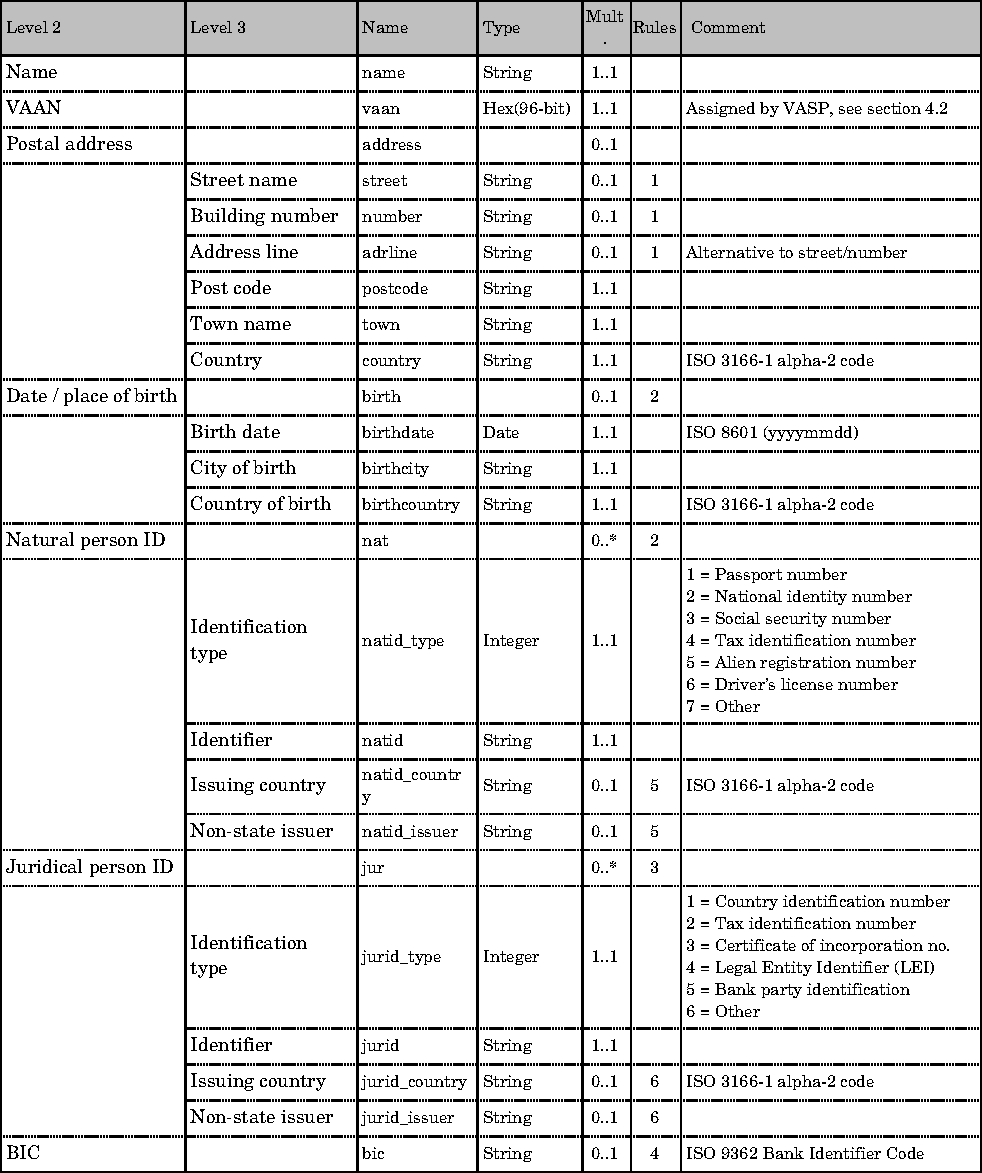
\includegraphics[width=\textwidth]{g28.pdf}
\end{figure}
\newpage
\subsubsection{Rules}
\begin{enumerate}
\item Either \verb+[street]+ and \verb+[number]+ must both be present or \verb+[adrline]+. All three positions can be present at the same time.
\item \verb+[birth]+ or \verb+[nat]+ is allowed, if neither \verb+[jur]+ nor \verb+[bic]+ is present.
\item \verb+[jur]+ is allowed, if neither \verb+[birth]+ nor \verb+[nat]+ nor \verb+[bic]+ is present.
\item \verb+[bic]+ is allowed, if neither \verb+[birth]+ nor \verb+[nat]+ nor \verb+[jur]+ is present.
\item If \verb+[nat]+ is present, either \verb+[natid_country]+ or \verb+[natid_issuer]+ or both must be present.
\item If \verb+[jur]+ is present, either \verb+[jurid_country]+ or \verb+[jurid_issuer]+ or both must be present.
\end{enumerate}
\newpage
\subsection{Beneficiary Information}
Mandatory and optional elements for transmitting originator data to be included in message types 210, 250, 310 and 350.
\begin{figure}[h]
    \centering
    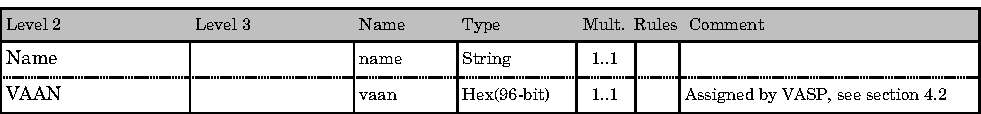
\includegraphics[width=\textwidth]{g29.pdf}
\end{figure}



\end{document}
